\documentclass[12pt,a4paper]{report}
\usepackage[a4paper,margin=1in]{geometry}
\usepackage[hidelinks]{hyperref}
\usepackage{caption}
\usepackage{graphicx}
\usepackage{lmodern}
\usepackage{setspace}
\usepackage{titlesec}
\usepackage{lipsum}
\usepackage{fancyhdr}
\usepackage{xcolor}
\usepackage{float}
\usepackage{tcolorbox}
\usepackage{amssymb}
\usepackage{amsmath}
\usepackage{algorithm}
\usepackage{algorithmic}
\usepackage{pifont}
\usepackage{booktabs}
\usepackage[Sonny]{fncychap}

\captionsetup{font=small}

\newcommand{\todo}[1]{%
  \par\noindent%
  \begin{tcolorbox}[colback=yellow, colframe=black, boxrule=0.5pt, sharp corners, width=\linewidth, before skip=5pt, after skip=5pt]
    \textbf{TODO:} #1
  \end{tcolorbox}%
  \par
}

\newcommand{\answer}[1]{%
  \par\noindent%
  \begin{tcolorbox}[colback=blue!10!white, colframe=blue!80!black, boxrule=0.5pt, sharp corners, width=\linewidth]
    \textbf{ANSWER:}~#1
  \end{tcolorbox}%
}

% REMARK (orange with ! icon)
\newcommand{\remark}[1]{%
  \par\noindent%
  \begin{tcolorbox}[ colback=orange!20!white, colframe=orange!80!black, boxrule=0.5pt, sharp corners, width=\linewidth, ]
    {\textbf{\textcolor{orange!80!black}!REMARK:}}~#1
  \end{tcolorbox}%
}

%--------------------------------
% Chapter Title
%--------------------------------
\ChNameVar{\raggedleft\bfseries\Large}   % "CHAPTER" word
\ChNumVar{\raggedleft\bfseries\Large}    % Chapter number
\ChTitleVar{\raggedleft\bfseries\Large}  % Chapter title

%--------------------------------
% Section Title
%--------------------------------
\titleformat{\section}[block]
    {\titlerule[2pt]\addvspace{0.8ex}%
    \bfseries\Large}
    {\thesection}{0.5em}
    {}[{\addvspace{0.4ex}\titlerule[2pt]}]
\titlespacing{\section}{0pt}{*4}{*4}

% Display current section in header:
\pagestyle{fancy}
\fancyhf{}
\fancyhead[L]{\nouppercase{\rightmark}}
\fancyfoot[C]{\thepage}

\begin{document}

% Title Page
\begin{titlepage}
    \centering

    % University logo at the top
    
\includegraphics[width=0.3\textwidth]{images/uantwerpen_logo.jpg}\\[1cm]

    {\Huge \textbf{Multimodal Data Integration for Predictive Modelling of Measles Vaccine Response with Cross-Vaccine Marker Validation}} \\
    \vfill

    {\Large \textbf{Elias Dams}}\\[1cm]

    \textbf{Promotor:} Dr. Pieter Meysman\\
    \textbf{Supervisor:} Fabio Affaticati\\[1.5cm]

    {\Large \textbf{University of Antwerp}}\\
    {\large Faculty of Science}\\[0.5cm]

    \textbf{2024-2025}\\[1.5cm]

    Submitted in fulfilment of the requirements for the degree of\\
    \textbf{Master in Computer Science: AI \& Data Science}\\[1cm]

    \textbf{June 2025}\\[2cm]

    % Decorative line at the bottom
    \vfill
    
\includegraphics[width=1.0\textwidth]{images/bottom_design.jpg}

\end{titlepage}

% remove page numbering
\pagenumbering{gobble}

% Table of Contents
\tableofcontents
\newpage

% List of Figures, Tables, Acronyms
\listoffigures

\listoftables

\chapter*{List of Acronyms}
- TCR: T-cell receptor

% Preliminary Sections
\chapter*{Summary}

\chapter*{Acknowledgements}

\chapter*{Abstract}




\chapter{Introduction}
% put page numbering back on
\pagenumbering{arabic}
\setcounter{page}{1}
%%%%%%%%%%%%%%%%%%%%%%%%%%%%%%%%%%%%%%%%%%%%%%%%%%%%%%%%%%%%%%%%%%%%%%%%%%%%%%%%%%%%%%%%%%%%%%%%%%%%%%%%%%%%%%%%%%%%%%%%%%%%%%%%%%%%%%%%%%%%%%%%%
% \todo{Introduce the research problem, significance of predictive modeling for vaccine response, and an overview of the multimodal data integration approach.}
% \remark{Maybe a citation here https://pmc.ncbi.nlm.nih.gov/articles/PMC5861809/} - Fabio

Vaccination is widely recognized as one of the most cost‑effective public health strategies, yet individuals exhibit significant variability in their immune responses. Foundational studies in systems immunology \cite{castrucci2018factors,brodin2017human} have shown that while vaccines like yellow fever and influenza generally trigger robust immune responses, the intensity of these responses (such as antibody production) can vary considerably. This variability is especially noticeable among very young or very old individuals, or those with other health issues, because their immune systems tend to be less robust and more unpredictable.\\
\\
%This thesis takes a data‑driven, computer science approach to predict responses to the measles (\remark{I would call it the MMR (Measles Mumps and Rubella trivalent vaccine, like you call it afterwards}Rubeola)
This thesis takes a data‑driven, computer science approach to predict responses to the MMR (Measles, Mumps, and Rubella) trivalent vaccine using multimodal data integration, meaning that it combines different types of data (each representing a distinct aspect of the immune response) into a single, unified analysis. In this thesis, the immune response is primarily evaluated based on antibody titers, which are regarded as the gold standard for assessing vaccine effectiveness because they offer a precise, quantifiable measure of the immune system’s capacity to generate protective antibodies \cite{plotkin2010correlates} (see Section~\ref{sec:antibody_titers} for further details). The goal is to develop predictive models that not only forecast individual measles vaccine responses but also identify specific immune markers that consistently correlate with vaccine effectiveness. Furthermore, aligning with the full scope of the thesis, a key objective involves cross-vaccine marker validation. This aims to assess whether markers predictive of the measles response are also indicates of immune response strength to different vaccines, specifically using data from a separate Hepatitis B vaccination study. Such cross-vaccine analysis is crucial for distinguishing between immune signatures specific to the measles vaccine and potentially universal markers associated with general vaccine-induced immune responses.\\
\\
Recent measles outbreaks in the United States and across Europe highlight the continued risk this highly contagious disease presents. Despite the widespread availability of an effective vaccine, factors such as declining vaccination rates in certain communities and the inherent variability in individual immune responses continue to contribute to the reappearance of measles \cite{Broom2025Measles,WHOEuropeUNICEF2025Measles,CDC2025MeaslesData}. The tragic consequences of these outbreaks, including hospitalizations and deaths, particularly among vulnerable populations such as young children, underscore the need for continued research to optimize vaccination strategies \cite{moss2017measles}. Predictive modeling is essential because it allows anticipation of an individual’s vaccine response well before the full immune reaction is measured. For example, Van Tilbeurgh et al. (2021) \cite{vanTilbeurgh2021predictive} demonstrated that combining high‑throughput technologies (such as transcriptomics, proteomics, and \textit{in vivo} imaging) with computational models can reveal immune signatures linked to vaccine efficacy. Such models support personalized vaccination strategies by allowing healthcare providers to tailor vaccine schedules, dosages, or even select alternative vaccines based on predicted responses. For example, if a model indicates a low immune response based on specific genetic markers, healthcare providers might opt for an additional booster or an adjusted formulation. Ultimately, this targeted strategy not only optimizes vaccine efficacy, but also ensures better resource allocation.\\
% \todo{@Fabio info about the study my data is coming from.}
% \remark{doi of the original study 10.1016/j.vaccine.2020.03.004} - Fabio
%The initial measles dataset used is derived from the study \remark{simply citing the first author and the date is fine} “Transcriptomic profiling of different responder types in adults after a Priorix$^{\mbox{\scriptsize\textregistered}}$ vaccination” \cite{bartholomeus2020transcriptomic}.
\\
The initial measles dataset used is derived from the study by Bartholomeus et al. (2020) \cite{bartholomeus2020transcriptomic}.
In this study, adult volunteers (23 females and 17 males, aged between 19 and 29 years, all of whom were previously primed with MMR vaccines in childhood) received a booster dose of Priorix$^{\mbox{\scriptsize\textregistered}}$ and were monitored at four time points (Day 0, Day 21, Day 150, and Day 365) to measure antibody titers and gene expression profiles. In this thesis, the focus will be concentrated specifically on the measles-related data from this dataset. \\
%For a detailed exploration of the dataset’s biological composition and characteristics, refer to Section~\ref{sec:biological_characterization_of_the_dataset}.\\
\\
Nevertheless, several challenges must be addressed to realize the full potential of predictive modeling. One challenge in this research is that the dataset comprises only 40 samples. This small sample size limits statistical power and increases the risk of overfitting, making it difficult to generalize the model to a broader population. In addition, the project involves integrating heterogeneous data types, such as cytokine levels, cytometry data, T cell receptor sequences, and RNA profiles. These different modalities come with varying scales and units, which adds complexity to data normalization and feature selection. In addition, any noise or missing values in a small dataset can have a large impact on the model’s performance, potentially leading to biased results. The high number of features (in the RNA data) relative to the number of samples may require careful feature selection or dimensionality reduction to prevent the models from becoming too complex and overfitted.
Finally, the objective of performing cross-vaccine marker validation introduces a specific challenge related to potential data leakage during feature selection. Methodologies must carefully ensure that information from the Hepatitis B dataset (e.g., test set performance or labels) does not influence feature selection or model training conducted primarily on the measles dataset (and vice versa). Such leakage could artificially inflate performance metrics and reduce the reliability of identified cross-vaccine markers.
%%%%%%%%%%%%%%%%%%%%%%%%%%%%%%%%%%%%%%%%%%%%%%%%%%%%%%%%%%%%%%%%%%%%%%%%%%%%%%%%%%%%%%%%%%%%%%%%%%%%%%%%%%%%%%%%%%%%%%%%%%%%%%%%%%%%%%%%%%%%%%%%%





\chapter{Background}
%%%%%%%%%%%%%%%%%%%%%%%%%%%%%%%%%%%%%%%%%%%%%%%%%%%%%%%%%%%%%%%%%%%%%%%%%%%%%%%%%%%%%%%%%%%%%%%%%%%%%%%%%%%%%%%%%%%%%%%%%%%%%%%%%%%%%%%%%%%%%%%%%
\todo{Cover key concepts in immunology and data science, review existing work on vaccine response modeling.}
\noindent
To understand the work presented in this thesis, it is essential to have a basic grasp of concepts from both immunology and data science. As a computer scientist, my approach is mainly data-driven, focusing on extracting, integrating, and analyzing various types of biological data. However, a foundational understanding of the underlying biological processes is critical to meaningfully interpret the results and validate the predictive models developed in this research.

\section{Background in Biology}

\subsection{Immune System Overview}

\begin{figure}[h]
  \centering
  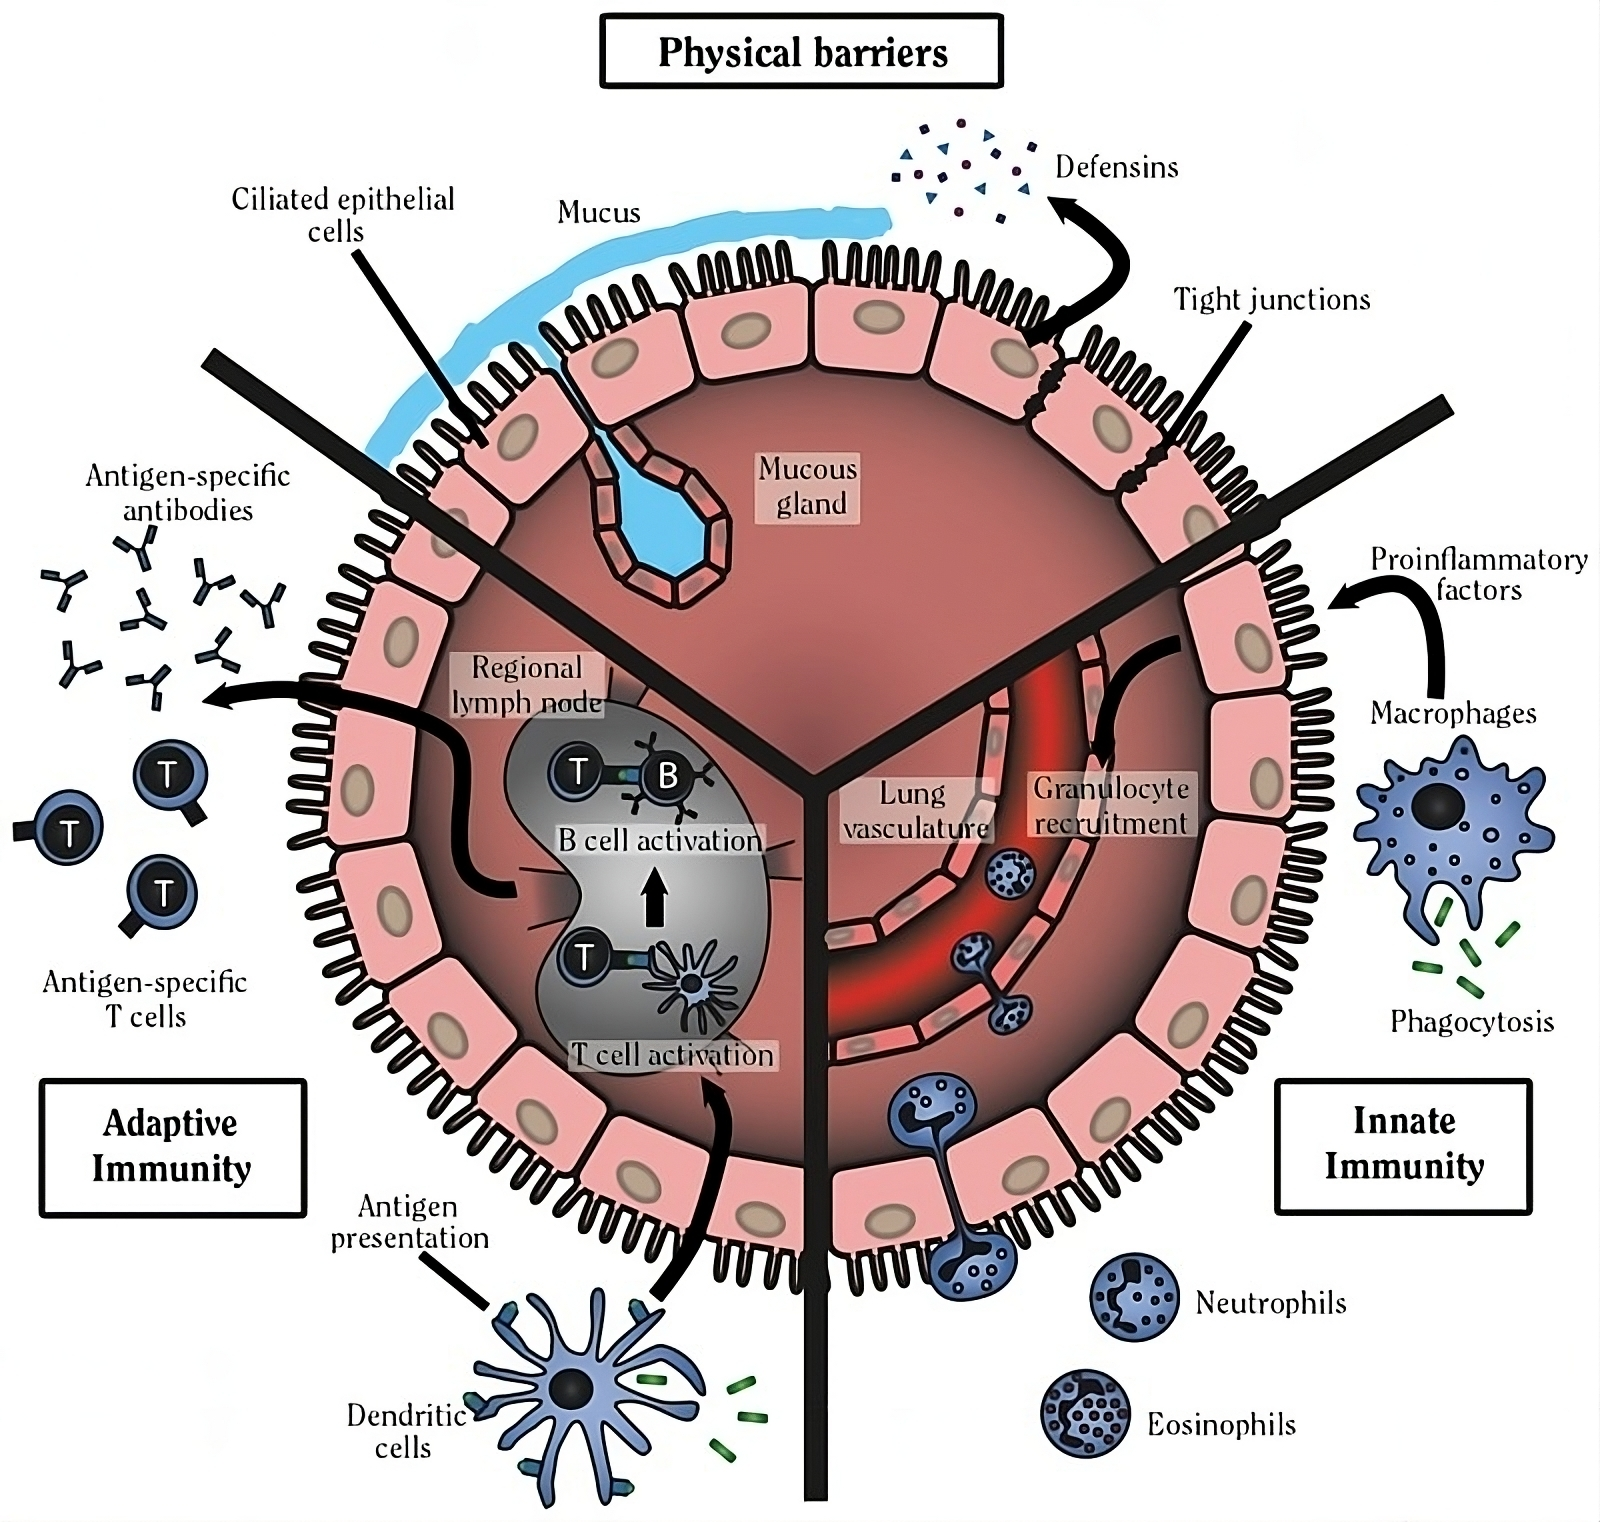
\includegraphics[width=0.9\textwidth]{images/Diagram_of_innate_and_adaptive_immunity.jpeg}
  \caption[Diagram of Innate and Adaptive Immunity]{Diagram showing physical barriers, innate immune cells (e.g., macrophages, dendritic cells, natural killer cells) and adaptive immune components (B and T cells) working together. Reproduced from Figure 10.5 in \emph{The Health Consequences of Smoking—50 Years of Progress: A Report of the Surgeon General} (2014) \cite{smoking2014}.}
  \label{fig:immunity}
\end{figure}
A key element of these biological processes is the functioning of the immune system, which can be broadly divided into three main components, as depicted in Figure \ref{fig:immunity}:\\
\\
\textbf{Physical barriers (top)}\\
Physical barriers, including the skin and mucous membranes, serve as the body’s first line of defense by blocking most pathogens (microorganisms such as viruses, bacteria, fungi, and parasites that can cause disease) from entering.\\
\\
\textbf{Innate Immunity (right)}\\
In case a pathogen still crosses the barriers, innate immunity comes into action. This defense is rapid and non-specific. Think of macrophages and neutrophils as cells that engulf invaders through a process called phagocytosis. Eosinophils and other granulocytes also attack pathogens or initiate inflammatory responses. Natural killer cells (NK cells) are also part of innate immunity and can directly destroy infected or abnormal cells. Although this response is very rapid, it does not recognize pathogens in the same specific way as the next branch. \cite{janeway2001immunobiology}\\
\\
\textbf{Adaptive Immunity (left)}\\
Acquired or adaptive immunity is the “slower but more targeted” defense. B cells play a crucial role by producing antibodies, which are proteins that bind to specific non-self antigens. These antibodies neutralize pathogens and tag them for destruction by immune cells such as phagocytes.
The concentration of these antibodies in the blood is measured as “antibody titers,” as mentioned earlier. Higher titers generally indicate a stronger immune response. T cells are also crucial and have several roles. They help coordinate the immune response (often referred to as “helper T cells”) and can directly kill infected cells (cytotoxic T cells). T cell receptors (TCRs), located on the surface of T cells and responsible for recognizing peptides presented by MHC I/II molecules, can be sequenced (see Figure\ref{fig:TCR_profiling}) to determine which T cell clones are activated in response to a vaccine. A major advantage of adaptive immunity is that it “learns” from previous exposure, allowing for much faster and more powerful immune responses in the event of repeated infection. This ability to form memory also underlies how vaccines work. \cite{janeway2001immunobiology}

\begin{figure}[h]
  \centering
  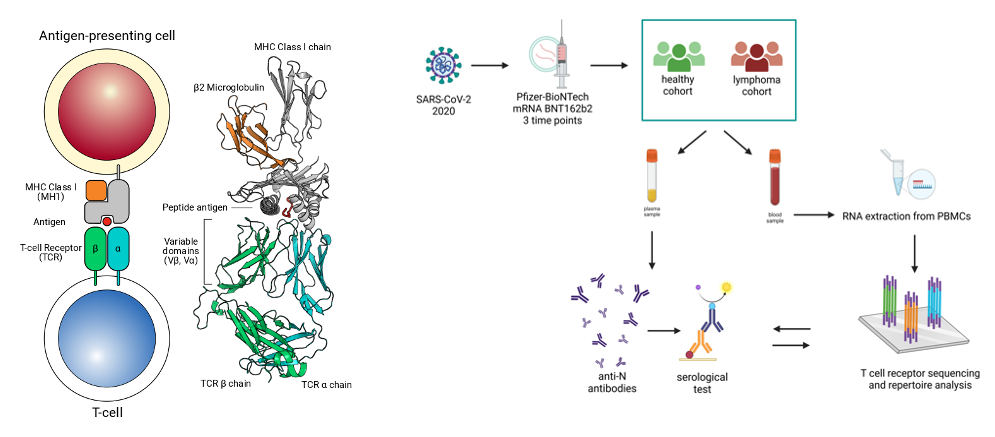
\includegraphics[width=1\textwidth]{images/TCR_profiling.png}
  \caption[ TCR sequencing Workflow]{Schematic outline of how TCR data is obtained from peripheral blood mononuclear cells (PBMCs) after vaccination. By extracting and profiling TCR sequences, it becomes possible to identify which T cell clones expand in response to the vaccine. This information provides insights into the breadth (diversity) and depth (magnitude or intensity) of the adaptive immune response.}
  \label{fig:TCR_profiling}
\end{figure}

\noindent
Together, these three pillars provide a robust defence system that is able to successfully fight off most infections. It is also this dynamic between innate and adaptive immunity that determines the degree of vaccine response. The innate branch prepares the way, while the adaptive branch provides targeted antibodies and memory cells. This context is important because the predictive models developed here integrate features from both the innate and adaptive immune systems. For example, innate markers such as cytokine levels and certain cell counts can provide early signals about the body's general readiness to respond. Meanwhile, adaptive markers, such as TCR sequences of T cells, directly reflect the specific immune response that leads to antibody production after vaccination. Combining this data gives us a more complete picture of the immune landscape, allowing for better predictions of how effectively an individual will respond to the measles vaccine.

\subsection{Antibody Titers}
\label{sec:antibody_titers}
As mentioned above, antibody titers provide a quantitative measure of the concentration of specific antibodies in the blood, making them a reliable indicator of the immune system’s functional response against a pathogen \cite{plotkin2010correlates}. In essence, they reflect the “signal strength” of the response, with high titers indicating robust protection and low titers suggesting a weaker response. In this thesis, antibody titers serve as a crucial biomarker for classifying vaccine responses into strong and weak responders.

\pagebreak
\section{Background in Computer science}
\todo{info about the used computer science techniques.}
\pagebreak
%%%%%%%%%%%%%%%%%%%%%%%%%%%%%%%%%%%%%%%%%%%%%%%%%%%%%%%%%%%%%%%%%%%%%%%%%%%%%%%%%%%%%%%%%%%%%%%%%%%%%%%%%%%%%%%%%%%%%%%%%%%%%%%%%%%%%%%%%%%%%%%%%





\chapter{Data Description and Preprocessing}
%%%%%%%%%%%%%%%%%%%%%%%%%%%%%%%%%%%%%%%%%%%%%%%%%%%%%%%%%%%%%%%%%%%%%%%%%%%%%%%%%%%%%%%%%%%%%%%%%%%%%%%%%%%%%%%%%%%%%%%%%%%%%%%%%%%%%%%%%%%%%%%%%
\todo{Detail the measles dataset (Cytokines, Cytometry, Clonal Breadth/Depth, RNA data) along with preprocessing steps taken.
Maybe i'll include a brief section here on hepatitis B preprocessing to set up the validation later.}
\noindent
In this chapter, I provide an overview of the measles dataset used in this study and outline the preprocessing steps required to prepare the data for analysis. The dataset integrates multiple biological modalities (including cytokine profiles, cytometry measurements, clonal breadth and depth of T cell receptors, and RNA sequencing data) to capture various aspects of the immune response to the measles vaccine. Additionally, I explain how response labels were assigned based on antibody titer trajectories, which serve as a key indicator of vaccine effectiveness.

\section{Label Assignment Strategy}
% \todo{@Fabio How where they initially defined to be sure? And also where it general antibody titers or specific to measles, because it it is specific a friend who studies biomedical science said that high titers over the whole trajectory should be considered "responder".  }
% \remark{They are specific to Measles (we also have the ABs for the other 2 components as well). The problem is that these individuals were already primed/they already had received a stimulation to the antigens before thus some had preexisting antibody titers but they didn't grow after vaccination thus technically not having a response to the stimulus. From the original paper: "For classification of the immune responses, a hierarchical clustering method was applied on the antibody (Ab) titers at day 0 (prevaccination baseline) and days 21, 150 and 365 (post-vaccination). This clustering technique groups individuals with similar patterns in Ab titer evolution. This avoids using cut-off values, which may be biased. As shown in Figure 2, four different response groups were identified for each antibody titer: 159 (a) High Ab: individuals with a relatively high Ab titer before vaccination that remained stable or further 160 increased after vaccination (b) Low Ab: individuals with a relatively low Ab titer before vaccination that remained low after vaccination (c) Long response: individuals with a relatively low Ab titer before vaccination that increased after vaccination and stayed stable within the first year (d) Peak response: individuals with a relatively low Ab titer before vaccination that increased at day 21, and then decreased by day 150 and 365."}

\noindent
Defining a successful immune response following vaccination can be complex, particularly in the presence of pre-existing immunity due to prior exposure or vaccination. To capture the dynamics of antibody levels over time, this study utilizes antibody titer measurements taken at four time points: Day0, Day21, Day150, and Day365.\\
\\
The original source study \cite{bartholomeus2020transcriptomic} employed a hierarchical clustering method based on these antibody titer evolution patterns to classify subjects into more granular response groups, effectively avoiding potentially biased arbitrary cut-off values. The study identified four primary response clusters: High Ab, Low Ab, Long response, and Peak response. For visualization purposes, these original classifications were consolidated into three categories displayed in Figure~\ref{fig:titer_original_label}: \texttt{responder}, \texttt{no response - high ab} (representing individuals with high baseline antibody levels who did not show a significant increase), and \texttt{no response - low ab} (representing individuals with low baseline levels who also did not show a significant increase).\\
\\
Figure~\ref{fig:titer_original_label} displays the antibody titer trajectories for each subject over the four measured time points, with lines colored according to these consolidated response categories. The x-axis represents the measurement day post-vaccination, while the y-axis indicates the antibody titer level. Each line follows the trajectory of an individual subject. The visualization highlights distinct dynamic patterns associated with these categories. Subjects classified as \texttt{responder} typically exhibit a pronounced increase in antibody titers following vaccination, primarily between Day 0 and Day 21, before a gradual decline. Conversely, the non-responder groups generally show more stable trajectories. The \texttt{no response - high ab} group maintains high titers throughout, while the \texttt{no response - low ab} group maintains low titers, neither showing the significant early boost characteristic of the responders. This visual distinction shows how pre-existing titers can influence the observed response pattern, where individuals with high baseline levels might not exhibit a noticeable increase even if they are protected.\\
\\
For the initial stages of predictive modeling in this thesis, we simplified the outcome variable to a binary classification: \texttt{responder} and \texttt{non-responder}. This simplification was made to create a more straightforward prediction task, focusing on the presence or absence of a successful boosting effect. Based on the visually distinct boosting pattern observed in Figure~\ref{fig:titer_original_label}, a subject was defined as a \texttt{responder} if their antibody titer increased by at least 120 mIU/mL from Day0 to Day21. This threshold reflects a widely accepted criterion for achieving protective immunity against measles \cite{chen1990measles} and corresponds to capturing the significant initial titer increase characteristic of the \texttt{responder} group in the figure. Subjects from both the \texttt{no response - high ab} and \texttt{no response - low ab} categories in Figure~\ref{fig:titer_original_label} were combined into the \texttt{non-responder} class for the binary prediction task, as neither group exhibited this defining boosting signature despite their different baseline states. The complexity and nuances captured by the original multi-class classifications will be considered for future modeling refinements or more detailed analyses.















% \begin{figure}[H]
% \centering
% \hspace*{-1cm}
% 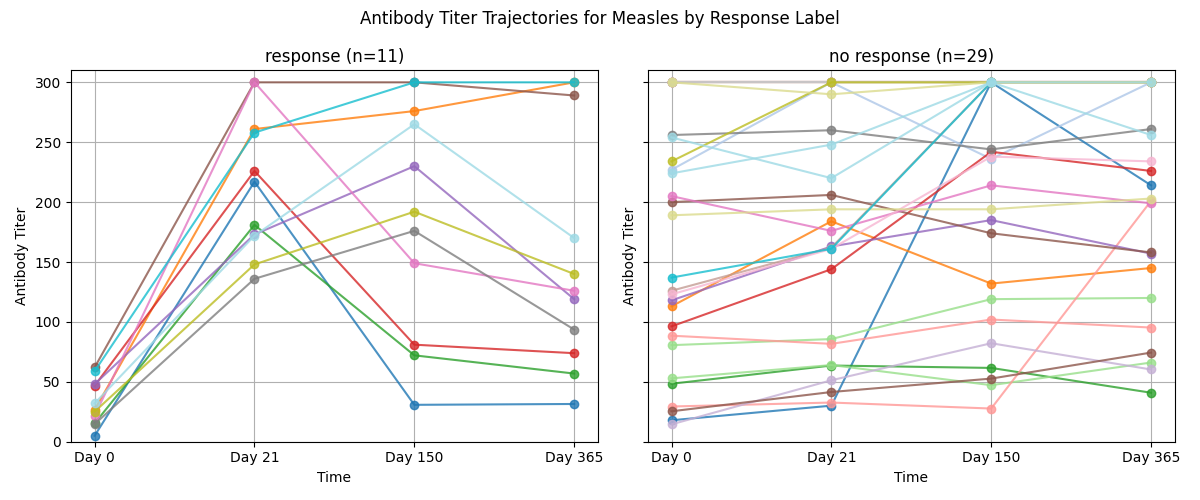
\includegraphics[width=1.1\textwidth]{images/Antibody_Titer_Trajectories_for_Measles_by_Response_Label.png}
% \caption[Antibody Titer Trajectories by Response Label]{Antibody titer trajectories for each subject, colored by final response label. Subjects labeled as \texttt{response} are shown in the plot on the left, while those labeled as \texttt{no response} are shown on the right.  The initial trajectory can be traced by following the color.}
% \label{fig:titer_response_label}
% \end{figure}

\begin{figure}[H]
\centering
\hspace*{-1cm}
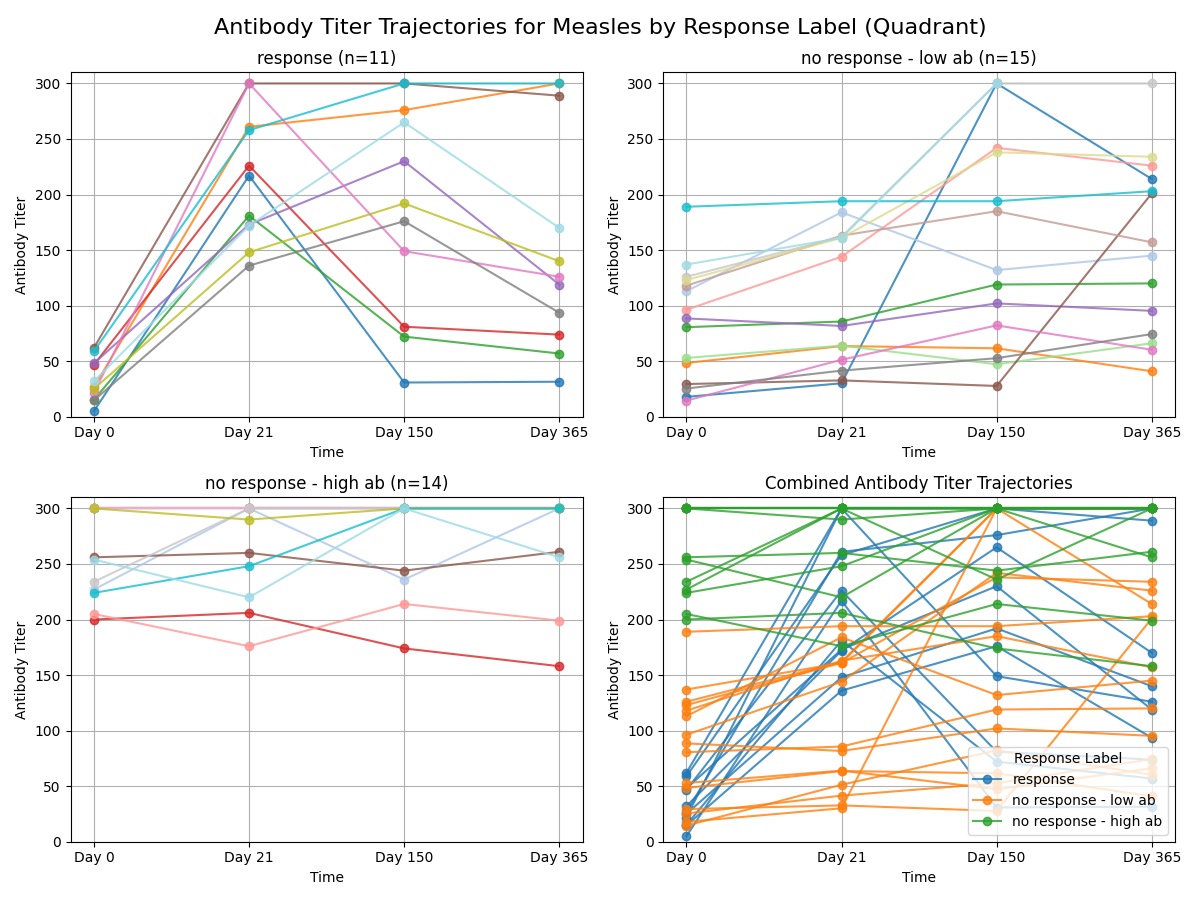
\includegraphics[width=1.1\textwidth]{images/Antibody_Titer_Trajectories_for_Measles_by_Original_Label_(Quadrant).png}
\caption[Antibody Titer Trajectories by Original Label (Quadrant)]{Antibody titer trajectories for each subject, colored by the original qualitative labels (quadrant). The plots show a clear differences in antibody responses, with responders displaying a sharp initial increase followed by gradual decline, while non-responders maintain consistently low or high titers.}
\label{fig:titer_original_label}
\end{figure}

\section{Dataset Construction and Preprocessing}
\todo{Explain the construction of TCR breadth and depth metrics, and describe the RNA data processing workflow. Ask @Fabio some questions about this!}

\pagebreak

\section{Correlation Analysis Within Individual Datasets}
\label{sec:correlation_analysis_within_individual_datasets}
\noindent
In an initial exploratory phase aimed at gaining familiarity with the data, preliminary analyses were conducted using Principal Component Analysis (PCA). This technique was applied to the full feature set, with a particular focus directed towards the cytokines dataset. Although this analysis was not a definitive or robust evaluation, it provided valuable insights by showing that the first 10 principal components captured the majority of the variance. This finding suggests that much of the dataset’s information can be summarized in fewer dimensions and indicates a high degree of redundancy among features. This observation led me to believe that similar correlations likely exist in the other datasets as well. Additionally, when I performed cross-validation using a Random Forest classifier on both the full and reduced feature sets, I observed that the balanced accuracy scores hovered near 50\%. The model tended to predict only the majority class, even though the overall accuracy appeared acceptable due to class predominance. These preliminary findings underscore the challenges of high dimensionality, multicollinearity, and class imbalance that need to be addressed in subsequent predictive modeling efforts.\\
\\
Following this, I delved deeper into understanding how the variables interrelate across the different data sources. As said earlier the study comprises five distinct datasets capturing various aspects of the immune response: cytokines, cytometry, clonal breadth (TCR metrics), clonal depth (TCR metrics), and RNA data. Since each dataset represents a unique facet of immunity, I investigated correlations within each individual dataset.  This strategy allowed me to uncover within-modality relationships, facilitating effective clustering of the data and providing the models with informative, explanatory features.
\subsection{Methodology}

\todo{Check if correct...}
\noindent
In my analysis, I use a Weighted Gene Co-expression Network Analysis (WGCNA) framework to identify modules of highly correlated features. First, I compute a correlation matrix from the data, which quantifies the pairwise relationships between features. This correlation matrix is then transformed into a distance matrix by taking one minus the absolute correlation value, ensuring that strongly correlated features are considered close. Instead of relying on a fixed linkage method like Ward.D2, WGCNA integrates hierarchical clustering with network analysis to detect modules, or clusters, of co-expressed features. In the implementation, I use the \texttt{flashClust} package for efficient hierarchical clustering, and then apply a dynamic tree cut procedure to define the modules. The modules are further visualized by assigning each a unique color using WGCNA’s labeling functions and displaying the resulting dendrogram and heatmap plots. This approach captures complex correlation patterns, effectively groups similar features.

\pagebreak
\subsection{Cytokine Data}
\begin{figure}[H]
  \centering
  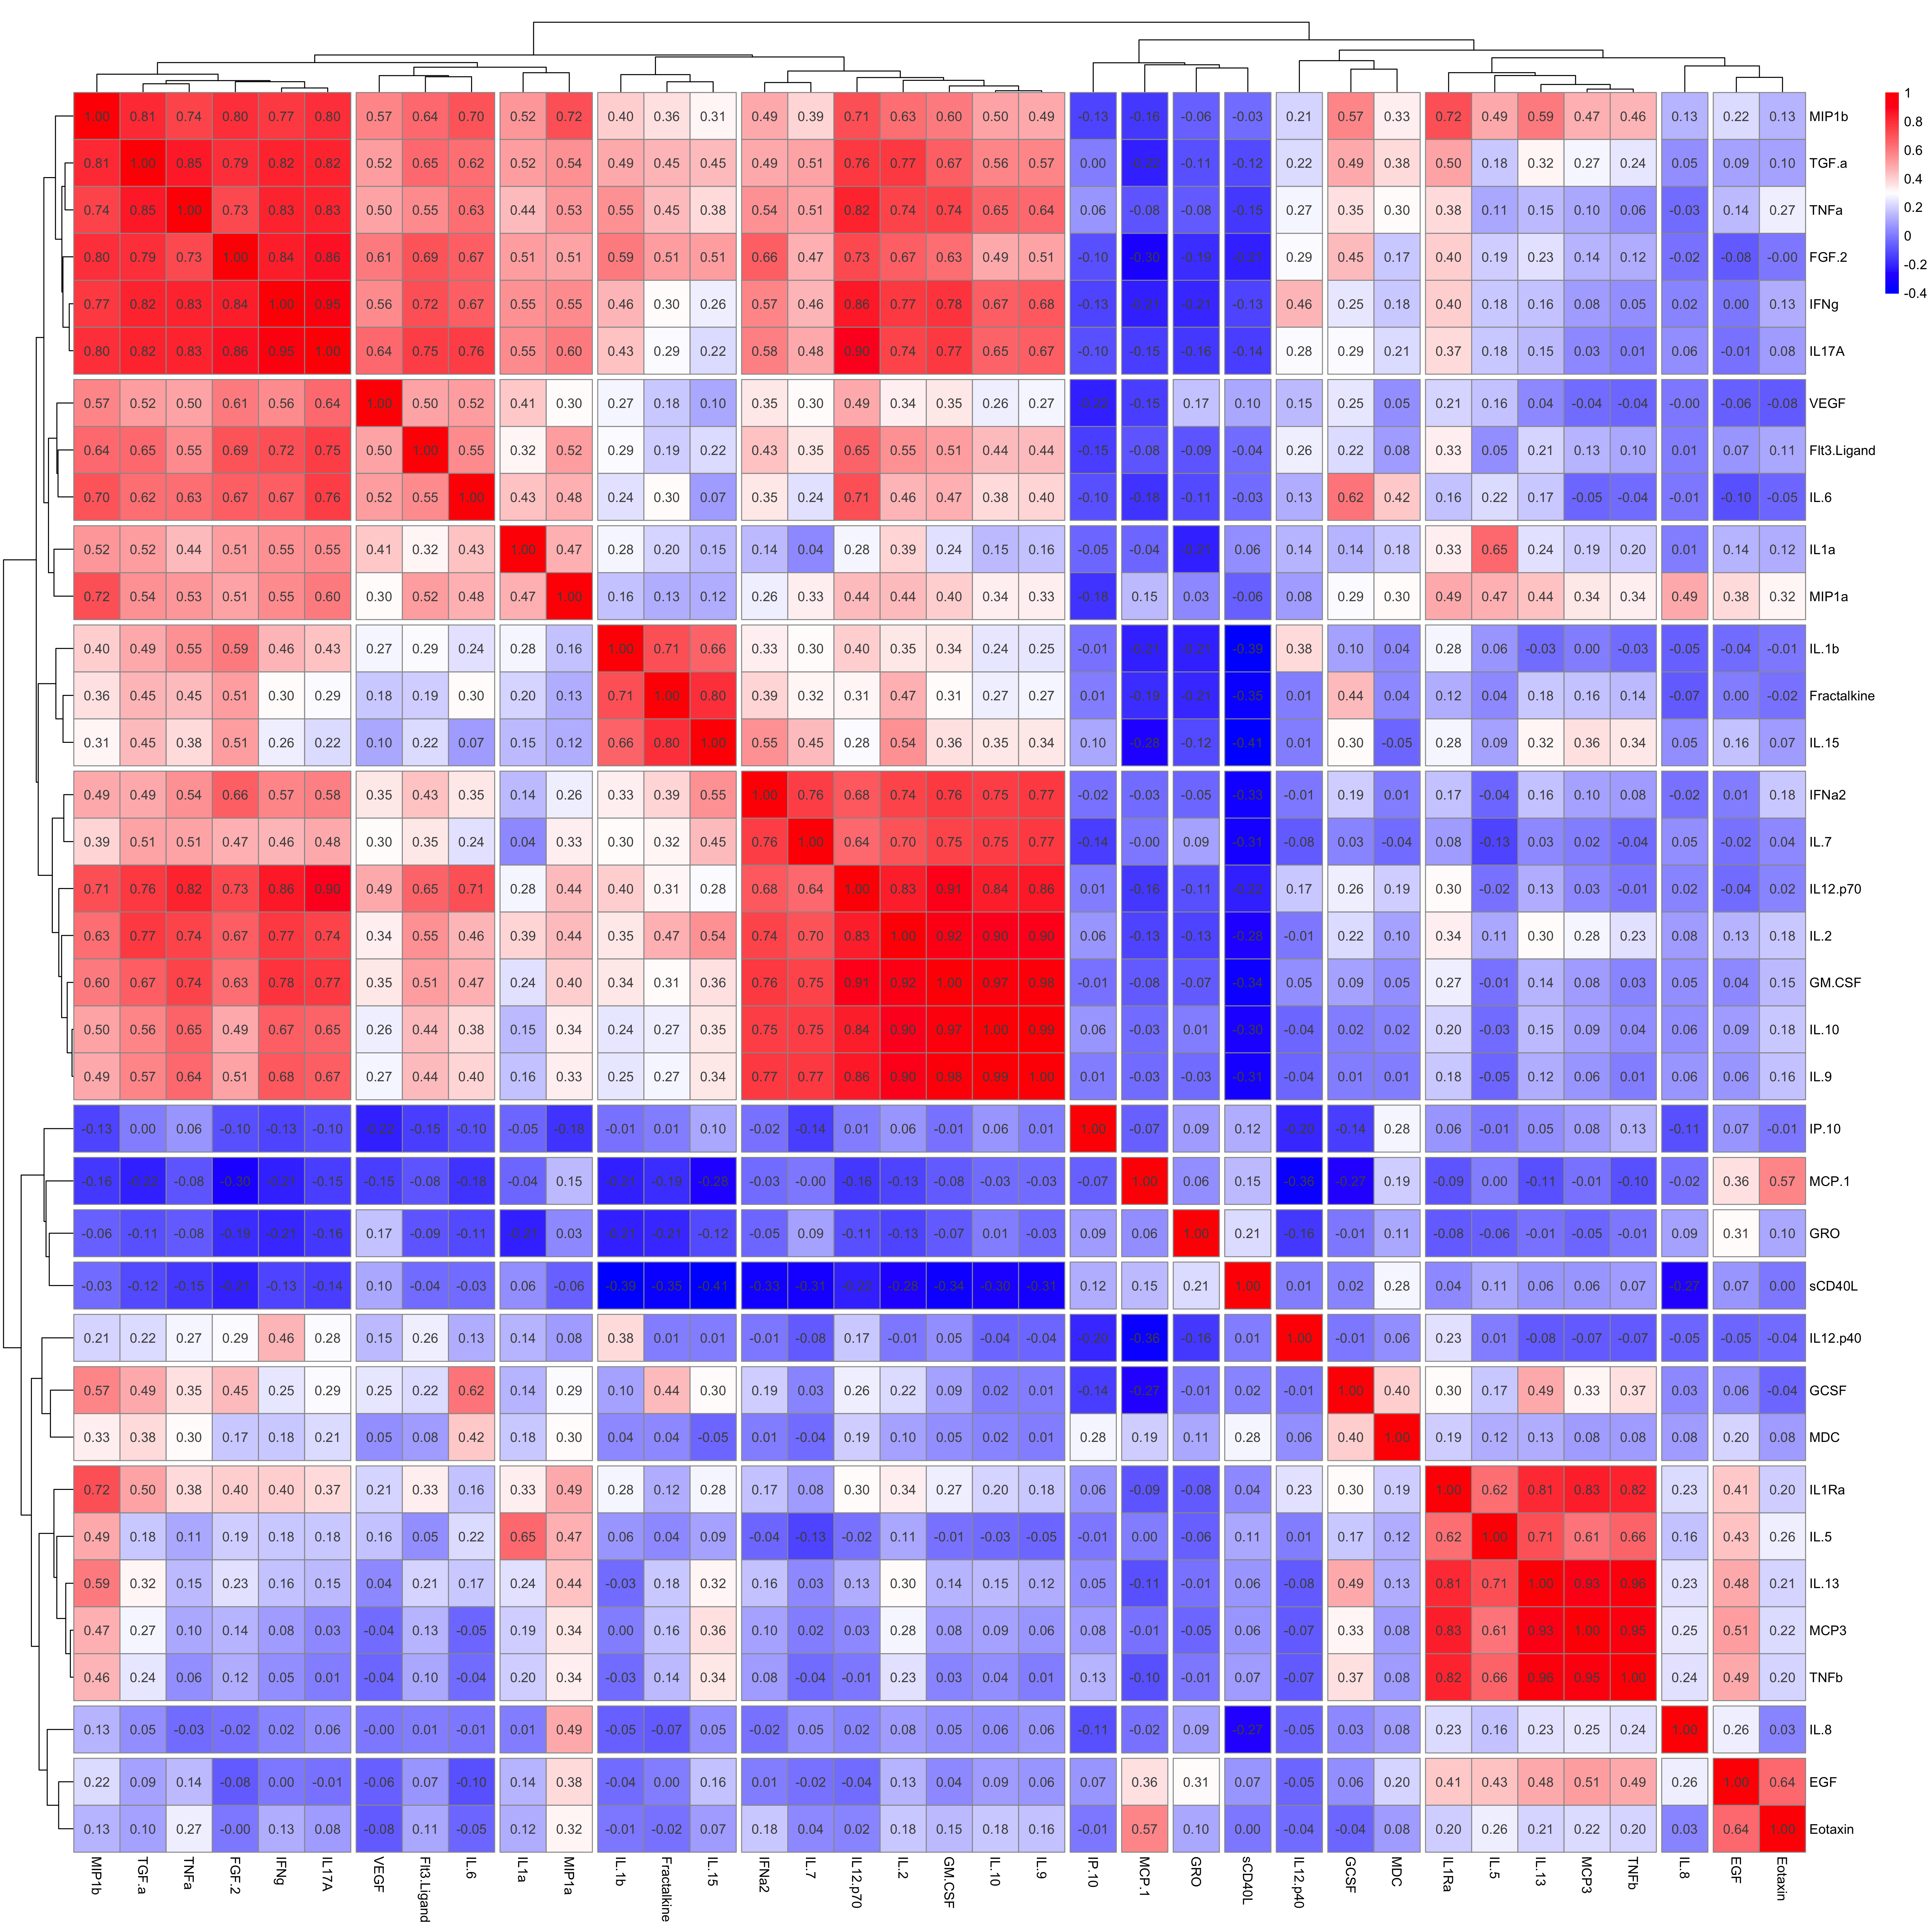
\includegraphics[width=0.8\textwidth]{images/Cytokine_euclidean_distance.png}
  \caption[cytokines data correlations]{Correlation heatmap of the cytokine data using  WGCNA hierarchical clustering.}
  \label{fig:cytokine_heatmap}
\end{figure}

The following cytokine clusters were obtained from the WGCNA hierarchical clustering analysis. The clustering reveals groups of cytokines with high inter-correlation, suggesting potential co-regulation or shared functional pathways.

\begin{table}[h!]
    \centering
    \begin{tabular}{ll}
        \textbf{Cluster 1:} & MIP1$\beta$, TGF-$\alpha$, TNF-$\alpha$, FGF-2, IFN-$\gamma$, IL17A. \\
        \textbf{Cluster 2:} & VEGF, Flt3 Ligand, IL-6. \\
        \textbf{Cluster 3:} & IL1$\alpha$, MIP1$\alpha$. \\
        \textbf{Cluster 4:} & IL-1$\beta$, Fractalkine, IL-15. \\
        \textbf{Cluster 5:} & IFN$\alpha$2, IL-7, IL12-p70, IL-2, GM-CSF, IL-10, IL-9. \\
        \textbf{Cluster 6:} & IL1Ra, IL-5, IL-13, MCP3, TNF$\beta$. \\
        \textbf{Cluster 7:} & GCSF, MDC. \\
        \textbf{Cluster 8:} & EGF, Eotaxin.
    \end{tabular}
    \caption{Cytokine Clusters}
    \label{tab:cytokine_clusters}
\end{table}


\subsection{Cytometry Data}

\begin{figure}[H]
  \centering
  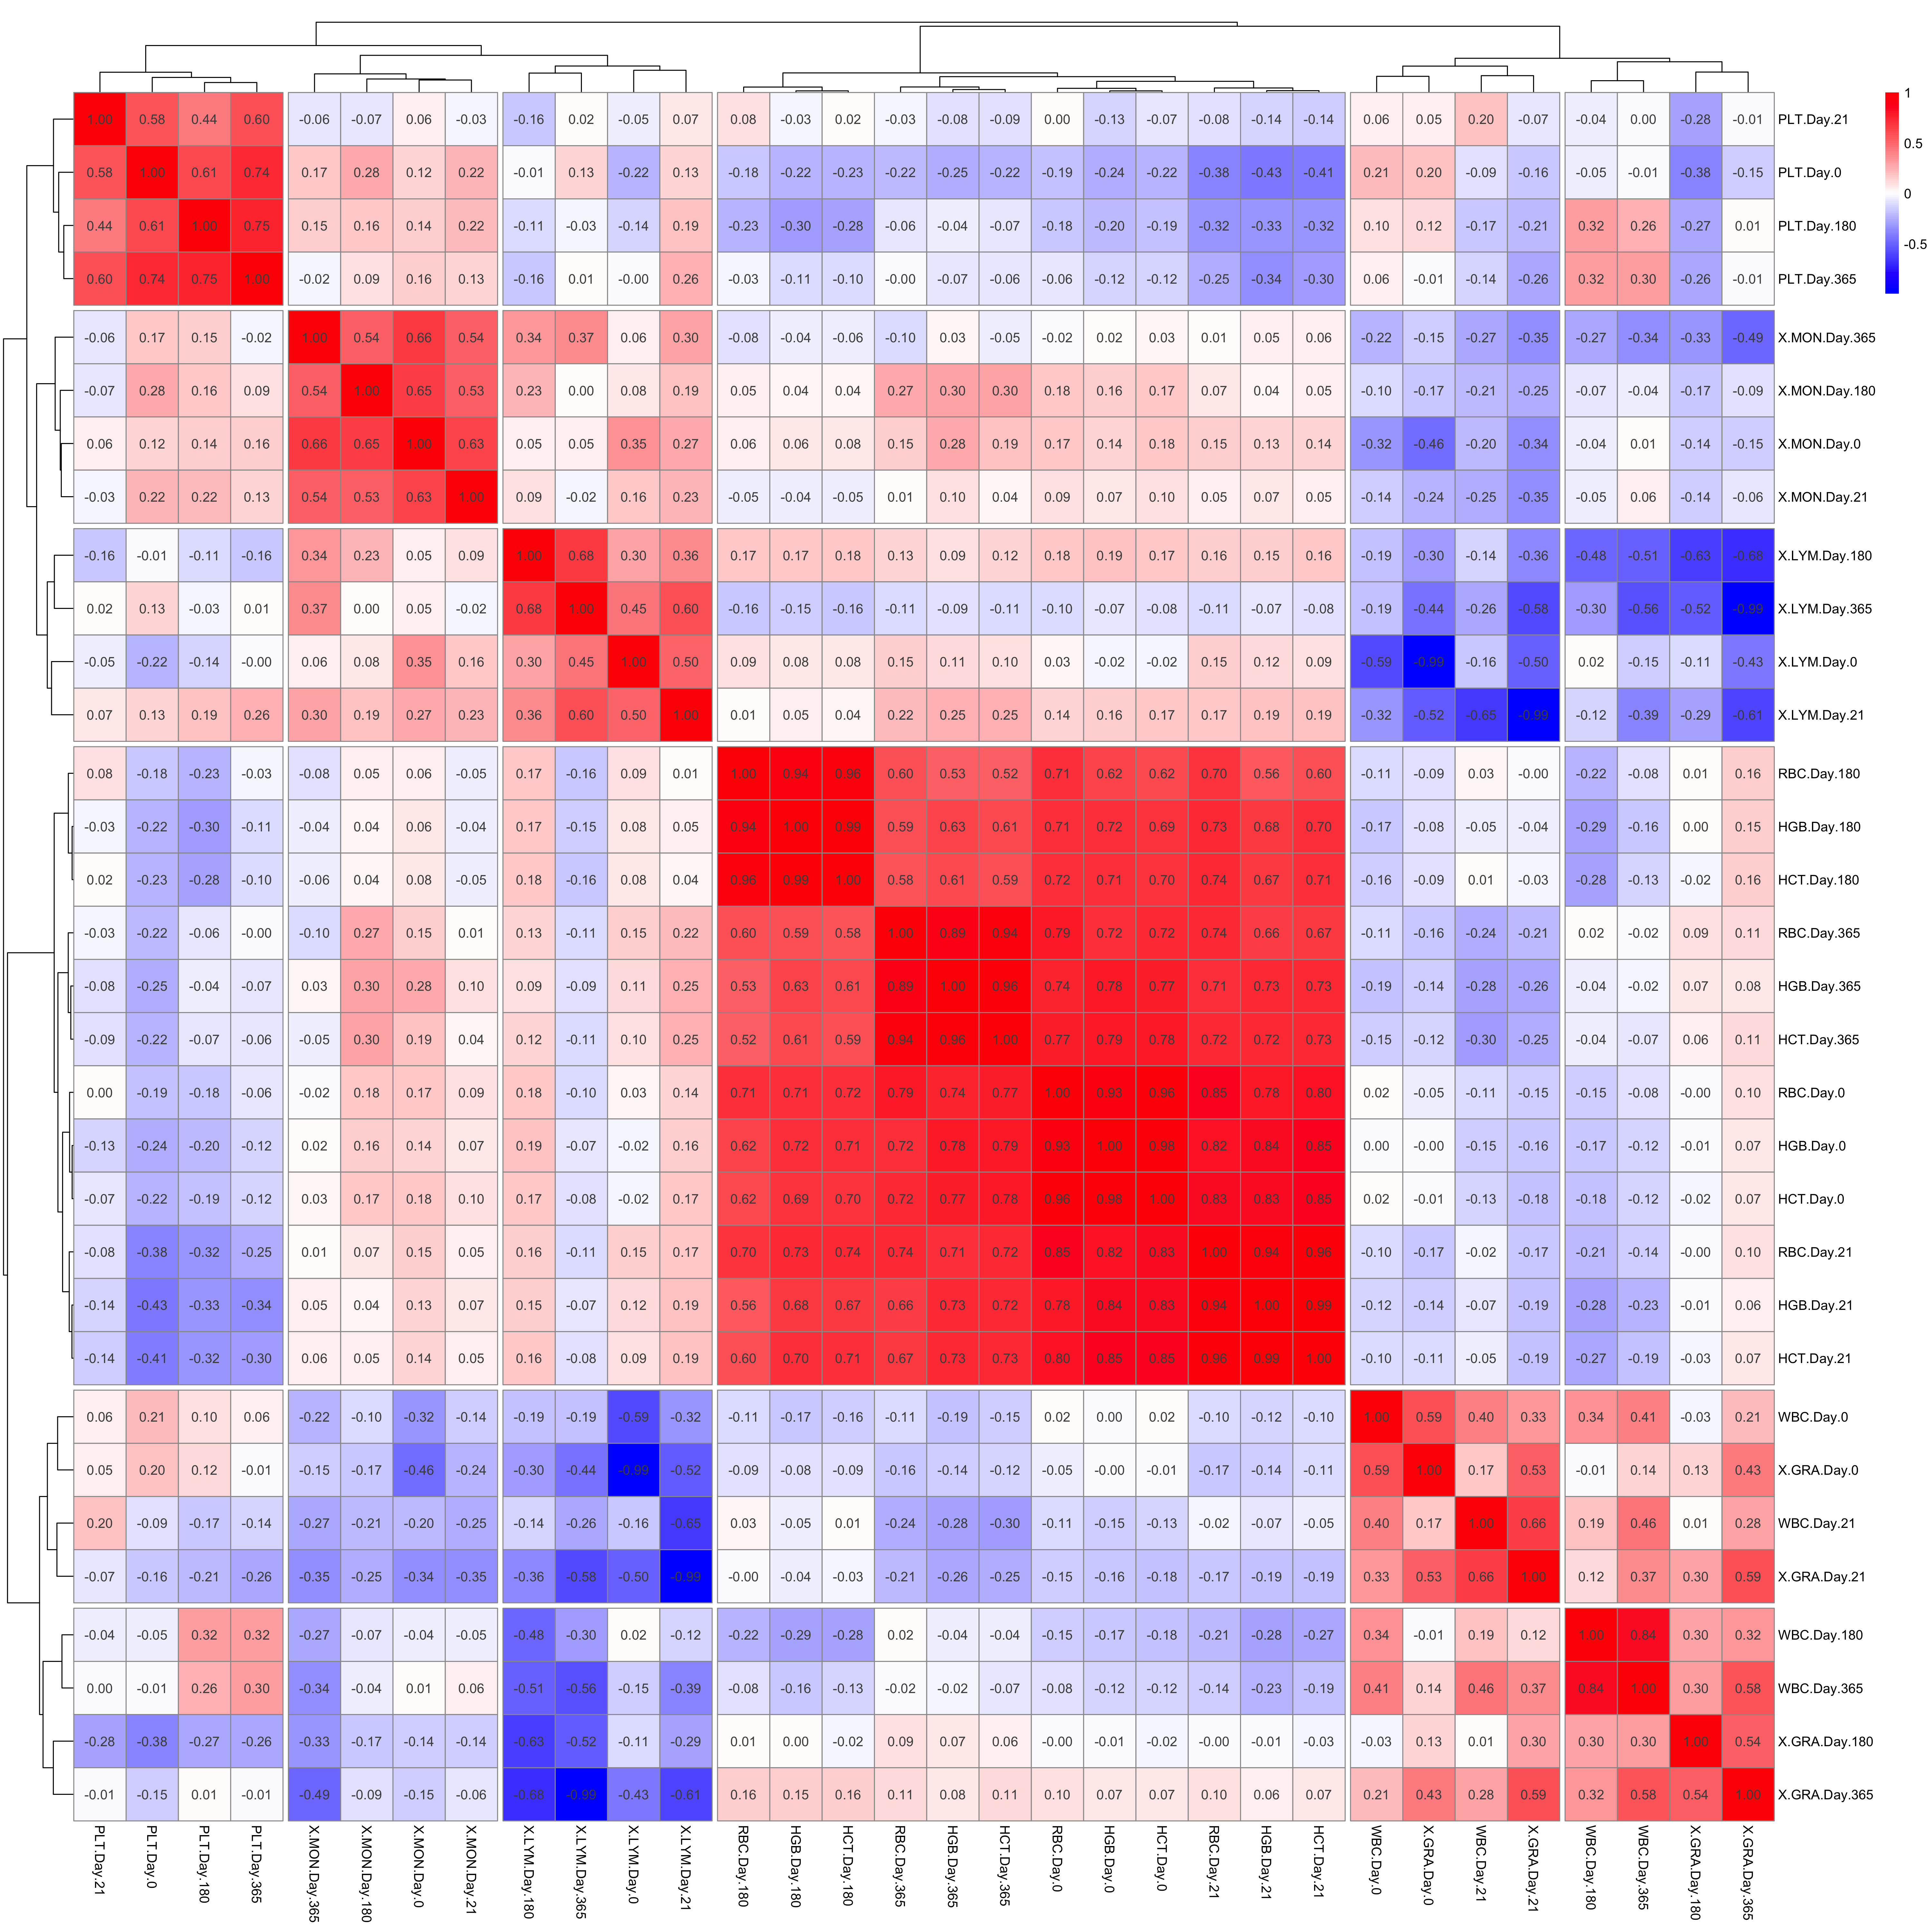
\includegraphics[width=0.8\textwidth]{images/Cytometry_euclidean_distance.png}
  \caption[cytometry data correlations]{Correlation heatmap of the cytometry data using  WGCNA hierarchical clustering.}
  \label{fig:cytometry_heatmap}
\end{figure}
\subsection{TCR Metrics}
\noindent
At Day~1, the heatmap reveals high correlation coefficients (e.g., 0.89--0.99) among RBC, HGB, and HCT, and similar correlation patterns emerge at Day~0, Day~21, Day~180, and Day~365, reinforcing their consistent co-variation over time. Even when only Day~1 is considered.
\begin{table}[h!]
    \centering
    \begin{tabular}{ll}
        \textbf{Cluster 1:} &  RBC, HGB, HCT
    \end{tabular}
    \caption{Cytokine Clusters}
    \label{tab:cytokine_clusters}
\end{table}



\subsection{RNA Data}
\begin{figure}[H]
  \centering
  \includegraphics[width=0.8\textwidth]{images/circos_RNA_only.png}
 \caption[RNA data correlations circular]{Circular correlation plot of the RNA data using. Each feature is represented along the outer edge, with colored lines indicating correlations between features (blue for positive correlations, red for negative correlations). The dense network of lines highlights the complexity of the dataset and the difficulty in visually identifying specific patterns or clusters.}
  \label{fig:RNA_circos}
\end{figure}


The RNA dataset presented a greater challenge for correlation analysis due to the high dimensionality, with a total of 382 features. To explore potential relationships within this data, I employed various visualization techniques, including the circular plot shown above.\\
\\
 Although the plot provides a comprehensive overview of all possible correlations, the dense web of lines makes it difficult to discern specific patterns or clusters visually. However, the primary advantage of this visualization is that it allows for the identification of broad trends and the detection of features that may be particularly well-connected or influential.

\begin{figure}[H]
  \centering
  \includegraphics[width=0.8\textwidth]{images/RNA_euclidean_distance.png}
  \caption[RNA data correlations]{Correlation heatmap of the RNA data using  WGCNA hierarchical clustering.}
  \label{fig:RNA_heatmap}
\end{figure}

\noindent
The same heatmap visualization technique as used before was applied to the RNA dataset, using a total of 36 cuts to correspond to the 36 different RNA modules identified through WGCNA hierarchical clustering. Selecting 36 cuts was challenging, but this number provided a reasonable balance between capturing distinct clusters and maintaining interpretability. The heatmap displays clear blocks of correlated features, with red indicating positive correlations and blue indicating negative correlations.
\todo{@Fabio - Do I include a huge table of the clusters, because that does not seem that usefull.}

\remark{I think you can put it in the supplemental}

%%%%%%%%%%%%%%%%%%%%%%%%%%%%%%%%%%%%%%%%%%%%%%%%%%%%%%%%%%%%%%%%%%%%%%%%%%%%%%%%%%%%%%%%%%%%%%%%%%%%%%%%%%%%%%%%%%%%%%%%%%%%%%%%%%%%%%%%%%%%%%%%%





\chapter{Methodology: Modeling and Feature Selection for Measles}
%%%%%%%%%%%%%%%%%%%%%%%%%%%%%%%%%%%%%%%%%%%%%%%%%%%%%%%%%%%%%%%%%%%%%%%%%%%%%%%%%%%%%%%%%%%%%%%%%%%%%%%%%%%%%%%%%%%%%%%%%%%%%%%%%%%%%%%%%%%%%%%%%
%\todo{Explain your pipeline for exploratory analysis, model building, and selection of stable predictive features, highlighting the specific challenges and how they were overcome.}
\section{Consensus Model Approach}
\label{sec:consensus_model_approach}
\noindent
In the initial phase of the modeling process, this study opted for a consensus model approach to leverage the complementary strengths of multiple predictive models. This technique involves training several distinct models independently on the different datasets and then concatenating their responses to form a unified prediction. The reason behind this approach is that different models may capture unique aspects of the data or be sensitive to different feature sets, thus enhancing the overall robustness and generalizability of the predictions.\\
\\
It is noteworthy that while many conventional consensus or ensemble learning strategies achieve diversity by applying different model algorithms or parameterizations primarily to a single dataset or variations thereof \cite{Rokach2010}, the approach adopted in this thesis introduces diversity fundamentally at the data level. Here, distinct modeling pipelines, each including internal model evaluation and selection, are applied independently to multiple, heterogeneous datasets (cytokines, cytometry, clonal breadth, clonal depth, RNA data), each representing a different biological viewpoint. Only after each pipeline generates its best prediction on the test set are these modality-specific outputs aggregated.\\
\\
By combining model outputs, the consensus approach aims to mitigate individual model biases and reduce the risk of overfitting, particularly given the high-dimensional nature and small size of the dataset. However, the complexity introduced by this approach requires careful consideration of how model outputs are integrated and evaluated.

\begin{figure}[H]
  \centering
  \hspace*{-0.9cm}
  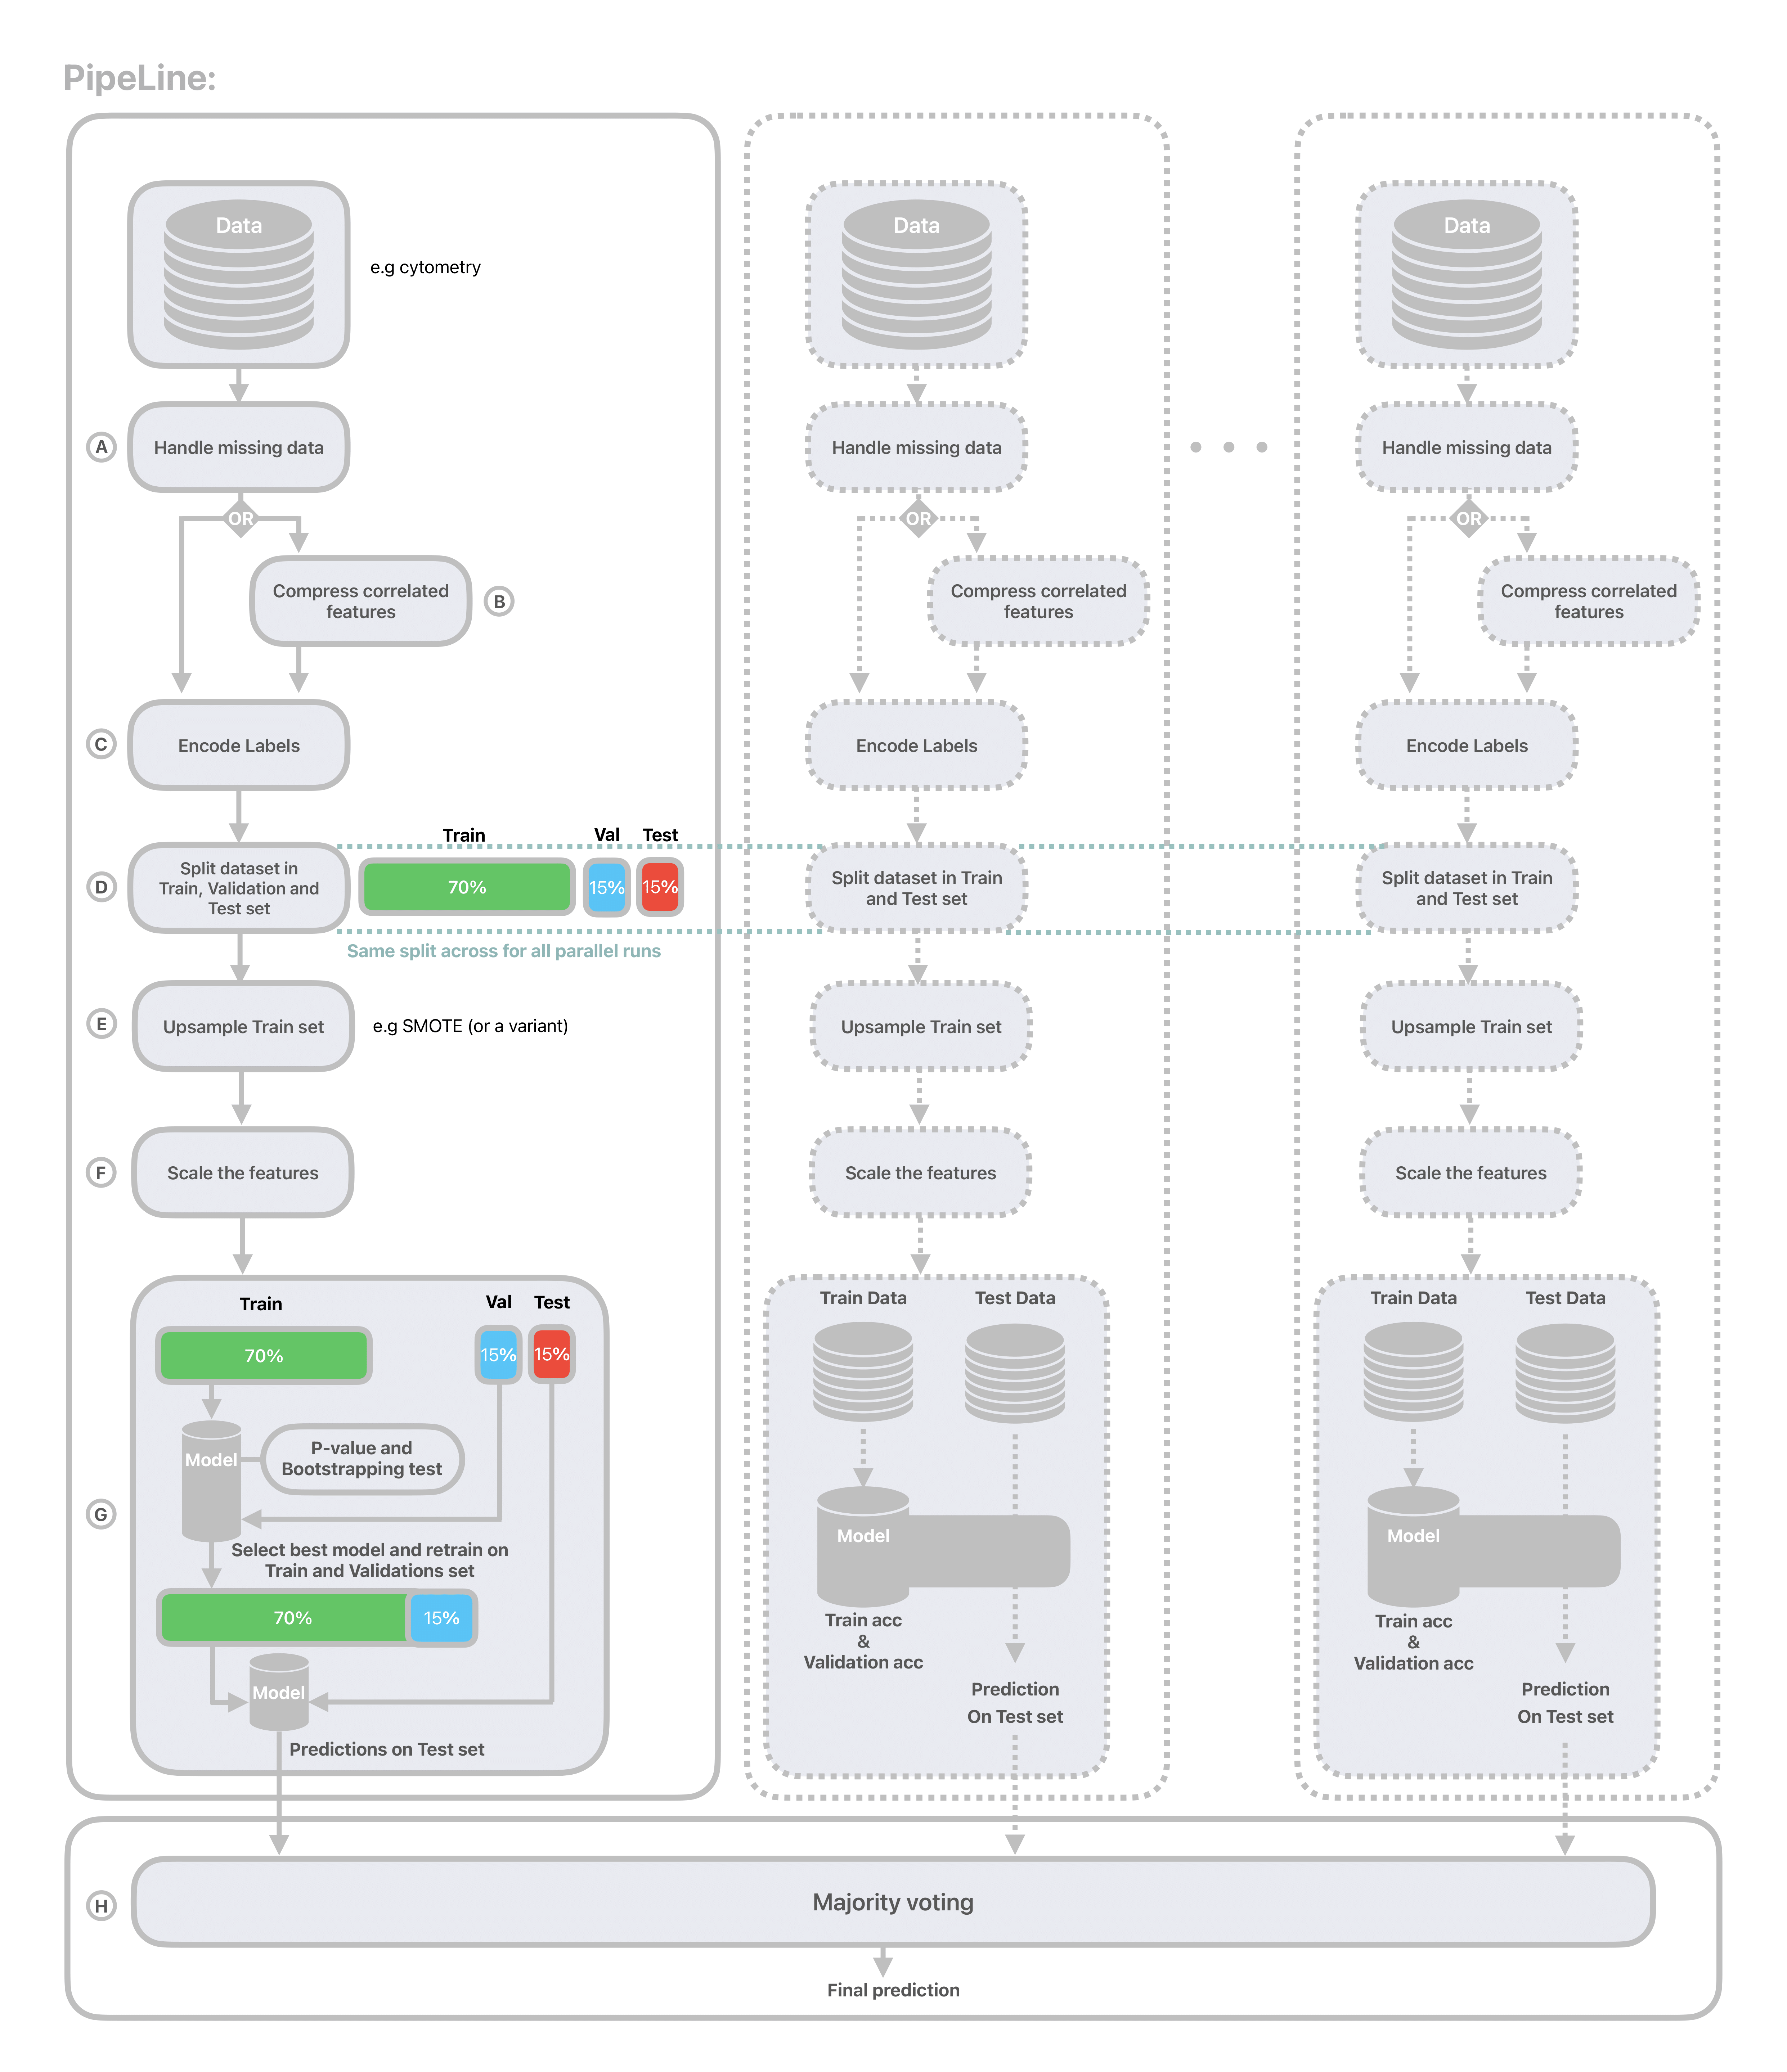
\includegraphics[width=1.1\textwidth]{images/Pipeline-1.png}
  \caption[Consensus model pipeline diagram]{The diagram illustrates the multi-model pipeline used for prediction. Each individual model follows a standardized preprocessing workflow: data loading, preprocessing (A: Missing data handling, B: Feature compression, C: Label encoding, F: Feature scaling), data splitting (D), upsampling the training set (e.g., using random upsampling or SMOTE) (E). The trained models then produce predictions, which are evaluated based on training, validation and testing accuracy. Additional validation is performed using p-value assessment and bootstrapping to ensure robustness (G). The final prediction is obtained through majority voting, aggregating predictions from all models to produce a consensus output (H).}
  \label{fig:pipeline-1}
\end{figure}

\subsection{Pipeline Structure for Heterogeneous Datasets}
\label{subsec:pipeline_structure_for_heterogeneous_datasets}
\noindent
This section details the structure applied within the consensus modeling framework. Specifically, five parallel pipelines were executed, each dedicated to one of the following distinct data types:
Cytokine measurements, Cytometry data, T-cell clonal breadth metrics, T-cell clonal depth metrics and RNA sequencing data.\\
\\
Although each pipeline starts with different data to capture unique biological insights, maintaining consistency across them is essential. Therefore, the same standardized workflow is applied to all five pipelines after loading their specific data. Using this uniform process ensures each distinct data type is handled the same before the final predictions are combined. As illustrated in Figure~\ref{fig:pipeline-1}, the standardized workflow applied to each dataset involves the following sequential steps:

\subsubsection*{Handle missing data \hyperref[fig:pipeline-1]{(A)}}
The initial step in the preprocessing pipeline involved a systematic check for missing values within the feature columns of each dataset. This is a standard procedure, as many machine learning algorithms require complete data matrices for training and prediction. Upon inspection of the datasets used in this study, no missing values were found within the feature columns relevant to the modeling process. Therefore, this step primarily served as a data integrity verification, and no imputation or sample removal actions due to missing feature values were necessary. (Handling of entire missing patient records for certain datasets was addressed during the data splitting phase as described in \textbf{{Split dataset(D)}}).

\subsubsection*{Compress correlated features \hyperref[fig:pipeline-1]{(B)}}
This pipeline step focuses on addressing highly correlated features within each dataset, based on the findings presented in Section~\ref{sec:correlation_analysis_within_individual_datasets}. To mitigate potential multicollinearity issues, these identified features were subsequently compressed into a single dimension using Principal Component Analysis (PCA), resulting in one principal component that represented them in the 'compressed' feature set.\\
\\
To investigate whether feature compression impacted the final consensus model's performance, the modeling pipeline following this step was executed using two parallel approaches for each dataset. One approach utilized the original, full set of features, while the other used the reduced feature set. While addressing correlated features can potentially reduce redundancy and improve model stability, the main purpose of this parallel analysis was to empirically determine if this compression step offered a measurable advantage to the predictive accuracy of the overall consensus model for each specific data type.

\subsubsection*{Encode labels \hyperref[fig:pipeline-1]{(C)}}
As machine learning algorithms typically require numerical inputs, the categorical target variable was converted into a numerical format in this step. This encoding simply assigned a unique integer (e.g., 0 and 1) to each response class.

\subsubsection*{Split dataset \hyperref[fig:pipeline-1]{(D)}}
To properly evaluate model performance and ensure generalization to new data, the dataset was partitioned into three independent subsets: a training set, a validation set, and a test set.\\
\\
The partitioning followed a 70\% / 15\% / 15\% ratio, allocating the data as follows:
\begin{itemize}
    \item \textbf{Training Set (70\%):} This largest subset was used solely for training the models. The algorithms learn patterns, relationships, and parameters from this data.
    \item \textbf{Validation Set (15\%):} This independent subset was crucial during the model development phase, specifically for selecting the optimal combination of model algorithm and data preprocessing choices. Since multiple distinct model types were evaluated in parallel across the pipelines, and different up-sampling techniques were considered (detailed in the next step), this validation set was used to compare their performance. The combination of model algorithm and up-sampling method yielding the best results on the validation set was selected for final evaluation. Performing the model and up-sampling selection using the validation set is critical to ensure that the test set remains completely untouched and unseen, thereby preserving its integrity for the final, unbiased assessment of generalization performance.
    \item \textbf{Test Set (15\%):} This subset was strictly held out until all model development and selection were finalized based on the training and validation sets. It was used only once at the very end to provide a final, unbiased estimate of how the chosen model configuration is expected to perform on new, unseen data.
\end{itemize}
\noindent
The datasets presented a challenge in terms of sample size consistency: cytokine, cytometry, and RNA data were available for all 40 patients, whereas clonal breadth and depth data were limited to 27 patients. Despite this discrepancy, evaluating the performance of each pipeline and, critically, aggregating their predictions for the final consensus model requires that all analyses utilize the exact same held-out test set. Maintaining this test set consistency across all data modalities was therefore essential for the validity of the study's comparative evaluations and the subsequent consensus aggregation via majority voting.

\begin{figure}[H]
  \centering
  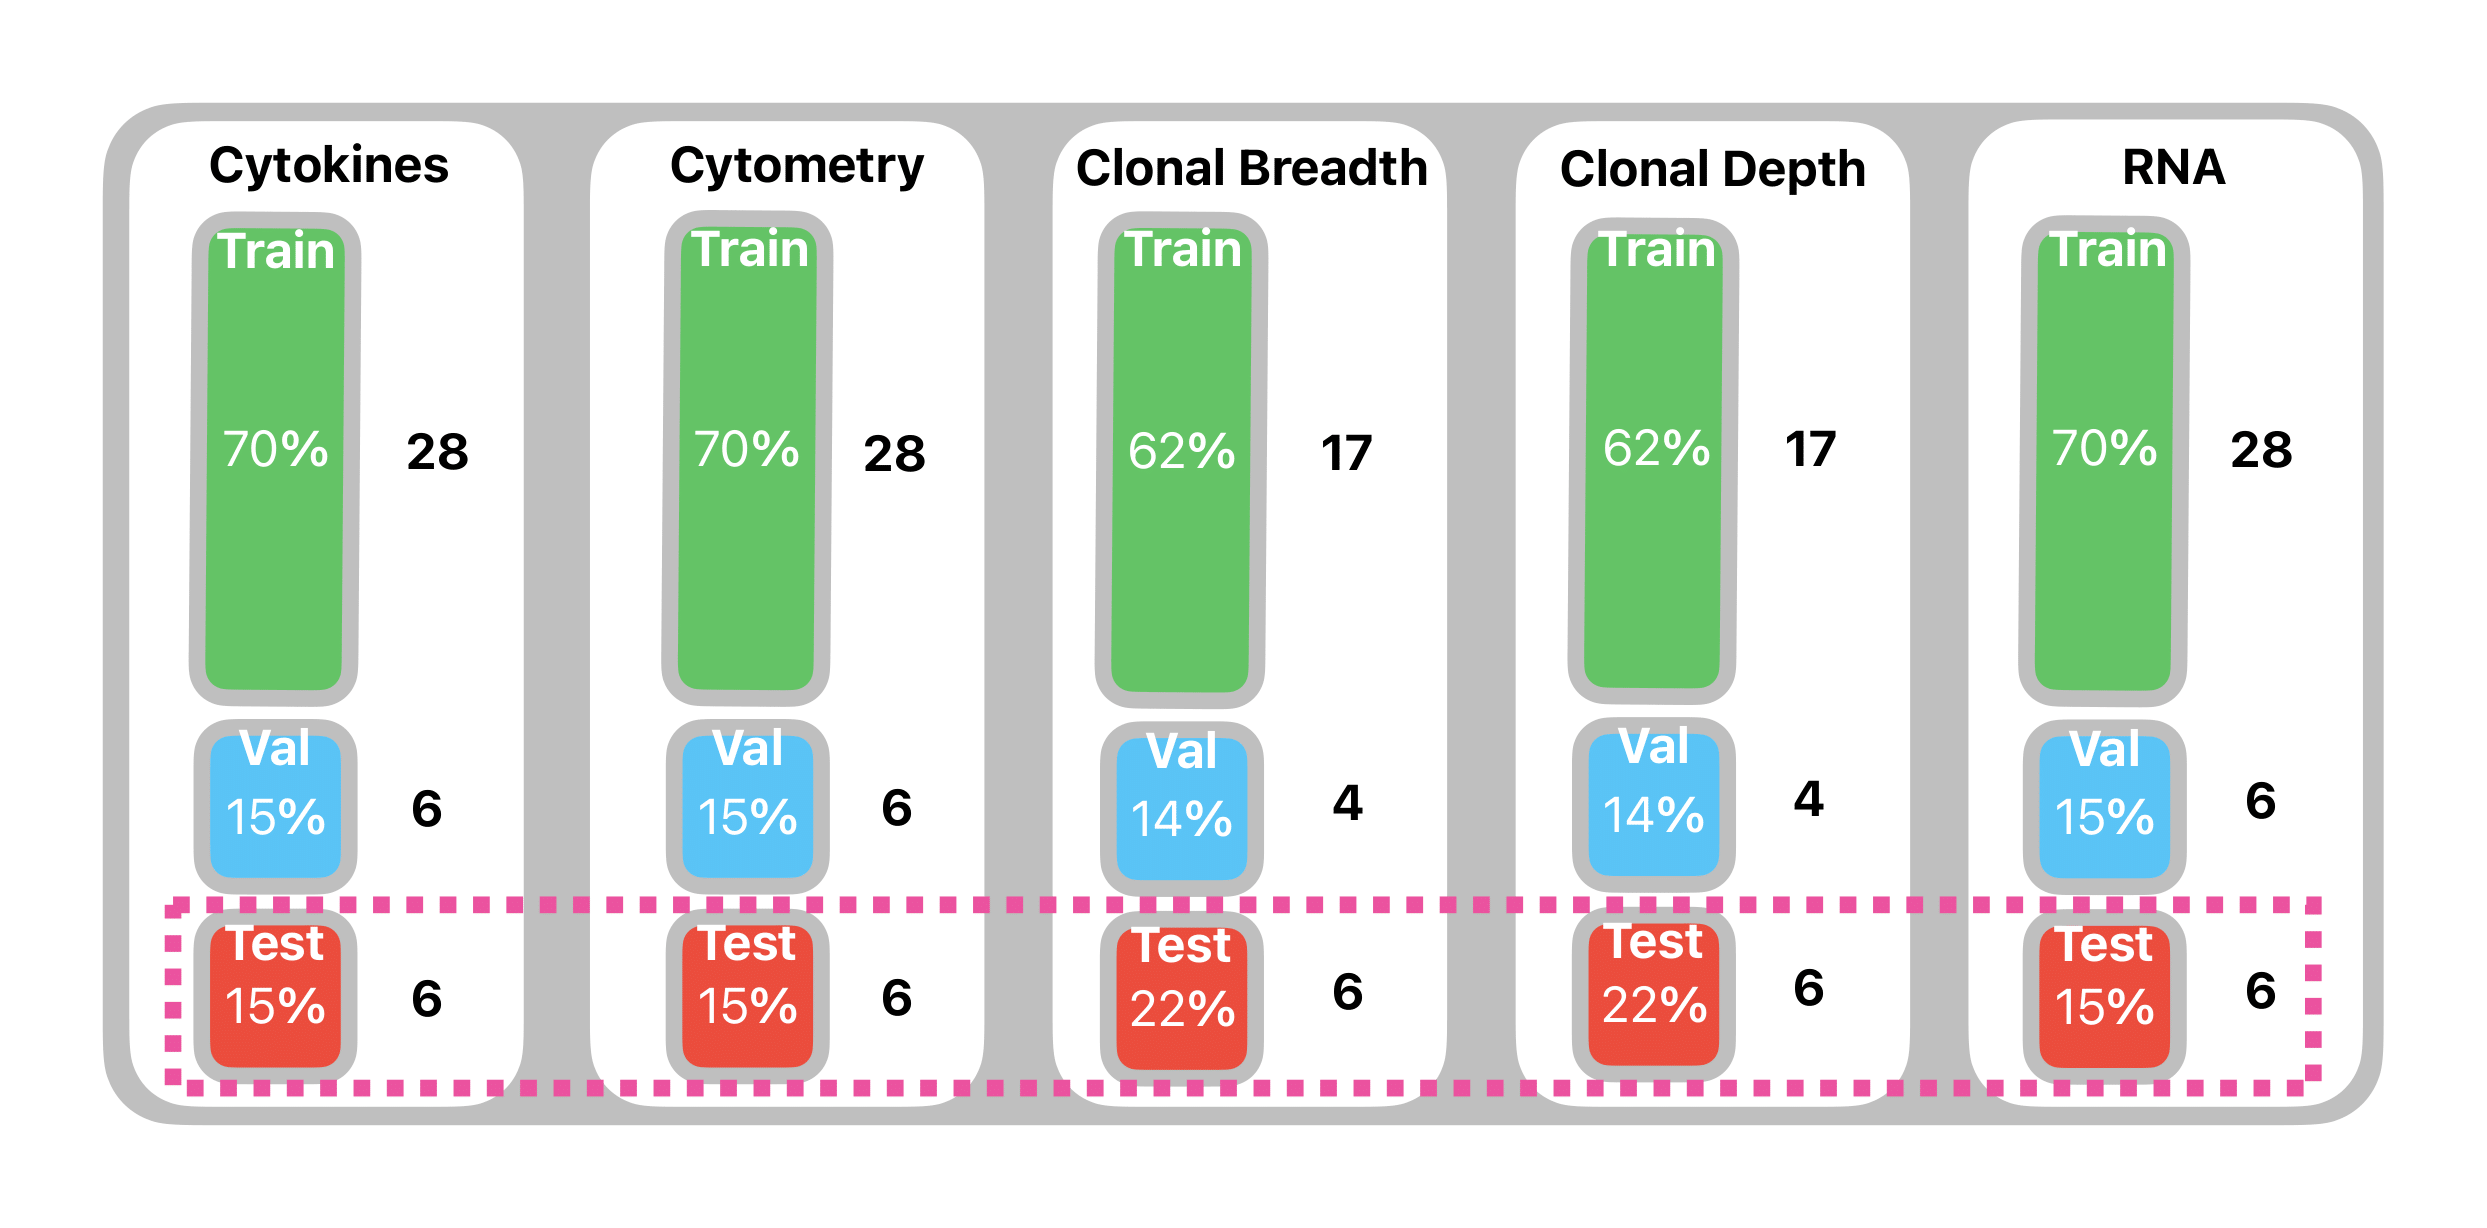
\includegraphics[width=0.8\textwidth]{images/split-1.png}
    \caption[Data splits per modality]{Visual summary of the Train/Validation/Test set splits applied to each data modality, showing sample counts and highlighting the consistent test set size (N=6).}
  \label{fig:split_data}
\end{figure}
\noindent
To achieve this, a global data partitioning strategy was defined based on the complete 40-patient cohort. A standard 70\% / 15\% / 15\% ratio was applied to this full cohort to designate specific individuals for the training (n=28), validation (n=6), and test (n=6) sets.\\
\\
This partitioning was applied directly to the complete datasets (cytokine, cytometry, RNA), resulting in the target split of 28/6/6. For the clonal depth and breadth datasets (N = 27), which represented subsets of the full cohort, a specific procedure ensured the consistency of the test set: the same 6 individuals designated globally for the test set were identified within the 27 available samples and assigned as the test set for these modalities. The remaining 21 samples specific to these datasets were then subsequently divided into training and validation sets, using an approximate 80\%/20\% split of this remainder, which resulted in 17 training samples and 4 validation samples for the clonal breadth and depth pipelines as can be seen in Figure~\ref{fig:split_data}.\\
\\
While this approach successfully maintained the crucial consistency of the test set across all analyses, it necessarily resulted in different effective sizes and ratios for the training and validation partitions in the clonal datasets (approx. 63\% Train / 15\% Val / 22\% Test) compared to the others (70\% Train / 15\% Val / 15\% Test). This variation was deemed an acceptable trade-off to preserve the integrity of the final, comparative evaluation on a common test cohort.


\subsubsection*{Up-sample Train set \hyperref[fig:pipeline-1]{(E)}}
\label{subsubsec:up-sample_train_set}
A common challenge in biological datasets is class imbalance, where one response class (in this case, responders) may be significantly less prevalent than the other within the training data. This may cause the model to favor the majority class during training. To counteract this and evaluate different mitigation approaches, three distinct strategies for handling class imbalance were applied exclusively to the 70\% training set:

\begin{enumerate}
    \item \textbf{No Resampling with Class Weighting:} In this strategy, the training data distribution was not modified. Instead, imbalance was addressed algorithmically during model training by assigning higher weights to the minority class samples. This typically adjusts the model's loss function, making errors on minority class examples more costly and forcing the model to pay more attention to them.
    \item \textbf{Random Over-Sampling (ROS):} This method directly modifies the training set by increasing the representation of the minority class. It works by randomly selecting and duplicating existing samples from the minority class until a desired level of balance (an equal number of samples per class) is achieved.
    \item \textbf{SMOTE (Synthetic Minority Over-sampling Technique):} Generating new, synthetic minority class samples through feature space interpolation, as detailed further below and illustrated in Figure~\ref{fig:SMOTE_explained}.
\end{enumerate}

\begin{figure}[htbp]
    \centering
    % Verify path is correct
    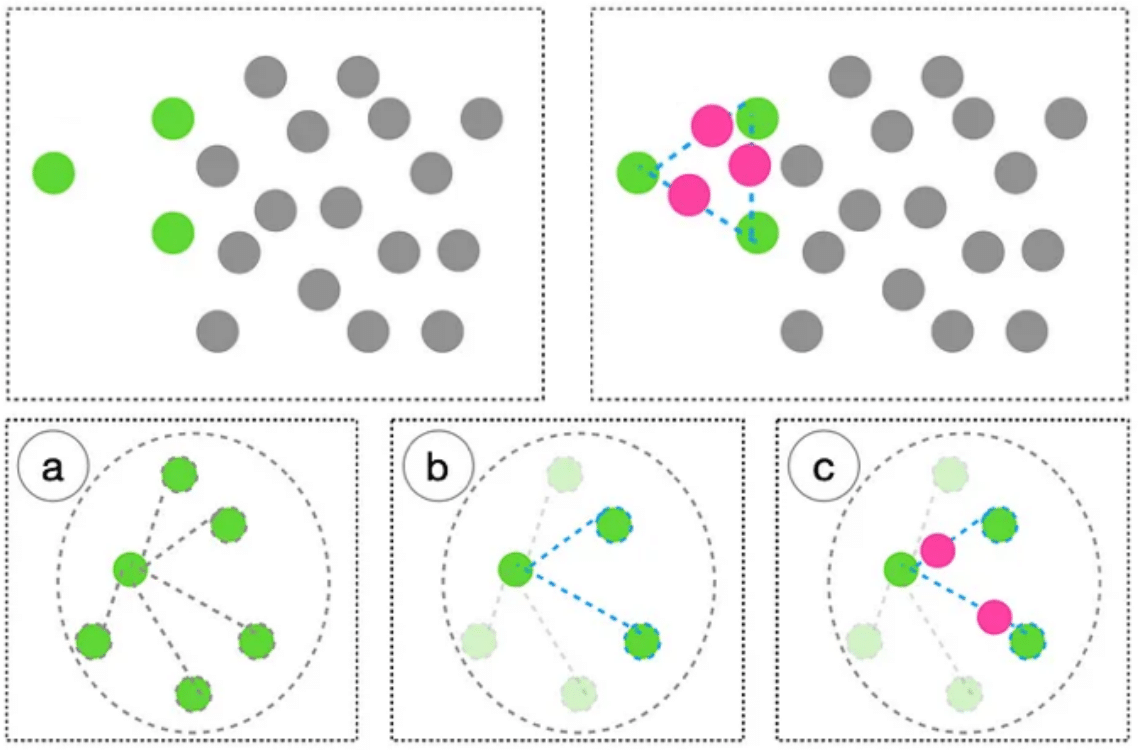
\includegraphics[width=0.8\textwidth]{images/SMOTE-explained.png}
    \caption[Illustration of the SMOTE mechanism]{Illustration of the Synthetic Minority Over-sampling Technique (SMOTE) mechanism. Top left: Initial imbalanced data distribution (minority in green, majority in gray). Top right: Generation of synthetic samples (pink) along lines connecting a minority instance to its nearest minority neighbors. Bottom row: Detailed steps showing (a) identification of k-nearest minority neighbors (here k=5), (b) selection of neighbors for synthesis, and (c) creation of synthetic samples (pink) along the vectors to selected neighbors. Figure based on figures 1 and 2 presented in \cite{Truong2022SMOTEVariants}.}
    \label{fig:SMOTE_explained} % Unique label
\end{figure}

\begin{figure}[htbp]
    \centering
    % Verify path is correct
    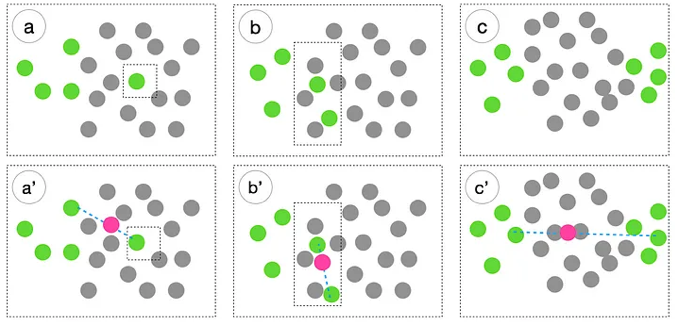
\includegraphics[width=0.8\textwidth]{images/SMOTE-weaknesses.png}
    \caption[Illustration of SMOTE weaknesses]{Conceptual illustration of potential weaknesses associated with SMOTE. The bottom row (a', b', c') depicts synthetic sample generation (pink) relative to regions shown in the top row (a, b, c). Potential issues illustrated include: (a/a') Generation influenced by potential noise or outliers (isolated minority sample). (b/b') Synthetic samples potentially overlapping with dense majority class regions due to disregard for majority sample proximity. (c/c') Generation possibly bridging distinct minority clusters, which could ignore underlying data structure or cause overgeneralization. Figure adapted from figure 4 presented in \cite{Truong2022SMOTEVariants}.}
    \label{fig:SMOTE_weaknesses} % Unique label
\end{figure}

\noindent
SMOTE \cite{Chawla2002SMOTE}, visually explained in Figure~\ref{fig:SMOTE_explained}, generates synthetic minority samples rather than simply duplicating existing ones like ROS. It selects a minority instance, finds its k-nearest minority class neighbors, and creates new samples along the line segments joining the instance to some of these neighbors. This method can potentially create a more diverse minority representation and smoother decision boundaries.\\
\\
However, SMOTE also has known limitations (illustrated in Figure~\ref{fig:SMOTE_weaknesses}), as discussed in literature \cite{Truong2022SMOTEVariants}. Potential drawbacks include overgeneralization (creating samples that blur class distinctions or ignore sub-clusters), amplification of noise if based on outlier samples, and possible generation of samples too close to or overlapping with the majority class, as the original algorithm doesn't explicitly consider majority proximity. Despite these points, SMOTE was included for comparison as a prominent synthetic data generation technique.\\
\\
The relative effectiveness of these three imbalance-handling strategies (Class Weighting, ROS, SMOTE) was assessed empirically for each model pipeline. As established during data splitting, the performance metrics achieved on the 15\% validation set were used to select the optimal strategy for each model before final assessment on the test set. It is crucial to mention again that these imbalance adjustments were applied strictly to the training data to maintain the integrity of the validation and test sets.


\subsubsection*{Scale the features \hyperref[fig:pipeline-1]{(F)}}
Feature scaling was applied to standardize the range of the input features. This ensures that features with larger values do not disproportionately influence distance-based or gradient-based machine learning algorithms. Using scikit-learn's `StandardScaler`, the features in the training set were scaled to have zero mean and unit variance. The parameters learned from the training set were then used to transform the validation and test sets consistently, preventing data leakage.


\subsubsection*{Train the models \hyperref[fig:pipeline-1]{(G)}}
\noindent
Following the comprehensive preprocessing stages (A-F) designed to prepare each dataset modality, the pipeline proceeds to the core modeling phase. The objective here is not necessarily to find a single universally best model through extensive tuning, but rather to train, rigorously evaluate, and select the most suitable baseline classification algorithm for each distinct pipeline configuration. That is, for each combination of initial dataset (e.g., cytokines, cytometry) and class imbalance handling strategy (weighting, ROS, or SMOTE). I also did an other run where i compressed the correlated features.\\
\\
A suite of five standard, well-established classification algorithms were employed as candidates within each pipeline shown in Table~\ref{tab:ml_models}. These models were generally used with default hyperparameters to provide a robust baseline comparison. If the class weighting strategy was selected in the preceding step, balanced class weights were incorporated into the algorithms during training.\\
\begin{table}[h!]
    \centering
    \scalebox{0.8}{%
    \begin{tabular}{lllll}
        \toprule
        Model & Configurations & & \\
        \midrule
        Random Forest (RF) & \textit{Default scikit-learn parameters}, & \texttt{random\_state=42}, & \\
        Logistic Regression (LogReg) & \textit{Default scikit-learn parameters}, & \texttt{random\_state=42}, & \texttt{max\_iter=1000} \\
        Support Vector Machine (SVM) & \textit{Default scikit-learn parameters}, & \texttt{random\_state=42}, & \texttt{probability=True} \\
        Decision Tree (DT) & \textit{Default scikit-learn parameters}, &  \texttt{random\_state=42}, & \\
        Gaussian Naive Bayes (NB) & \textit{Default scikit-learn parameters},  & & \\
        \bottomrule
    \end{tabular}}
    \caption[Machine Learning Models Used]{Machine Learning Models Used and their Configurations}
    \label{tab:ml_models}
\end{table}
\\
\noindent
The process of identifying the best model for each configuration began with training each candidate algorithm on its corresponding partition of training data (70\%). Following this initial training, the intrinsic stability and statistical significance of the model were rigorously assessed using the training data itself. Performance stability was evaluated through repeated 5-fold stratified cross-validation (n = 1000 repetitions), a procedure illustrated in Figure~\ref{fig:Bootstrapping-1}. This yielded a mean performance score and confidence intervals, providing insight into the robustness of the model's performance against variations in the training data splits. The statistical significance of this performance, relative to chance, was then determined using permutation tests (n = 1000 permutations), as shown in Figure~\ref{fig:P-value_test-1}. This test resulted in a p-value, quantifying the likelihood that the observed cross-validation performance could have arisen simply due to random chance.\\
\\
Although these initial evaluations provided valuable insights into model characteristics on the training distribution, the definitive selection of the optimal model for the specific pipeline was driven by performance on the independent 15\% validation set. Each trained candidate model generated predictions for the validation set samples, and a composite score (derived from the weighted F1-score and balanced accuracy) was calculated. The algorithm that achieved the highest composite score on the validation set was selected as the preferred model for that configuration. In the event of ties in the composite score (partly due to the very low sample size), the mean cross-validation score and subsequently the permutation test p-value (both derived from the training set evaluations) served as hierarchical tie-breakers.\\
\\
Once the best model algorithm was identified for a given configuration (e.g., SVM selected for Cytokine data processed with SMOTE and PCA), it underwent a final retraining step. This involved re-fitting the selected model architecture using a combination of the 70\% training partition and the 15\% validation partition. By retraining on this larger (85\%) dataset, the final model could potentially learn a more refined parameterization before deployment on unseen data. Finally, this fully trained model was applied to the completely untouched 15\% test set to generate the ultimate predictions for that specific pipeline configuration. These test set predictions were used in the final step to combine results from all the different model pipelines.\\
\\
This entire process (preprocessing, training, evaluation, selection, retraining, prediction) was executed in parallel for all configurations being tested (e.g., for cytokines with weighting, cytokines with ROS, cytokines with SMOTE, potentially repeated with/without PCA, and similarly for cytometry, clonal breadth, etc.). This resulted in multiple sets of predictions for the same test set, each derived from the best model identified for a specific pathway. These multiple prediction sets then serve as the input for the final consensus aggregation step, described next.

\subsubsection*{Consensus model\hyperref[fig:pipeline-1]{(H)}}
Finally, to produce the single output prediction of the overall consensus model, the predictions generated for the test set by each of the parallel pipeline configurations were aggregated. This aggregation was performed using "Majority Voting". For every sample in the test set, the class label predicted most frequently across all contributing pipeline models was selected as the final consensus prediction.

\begin{figure}[H]
  \centering
  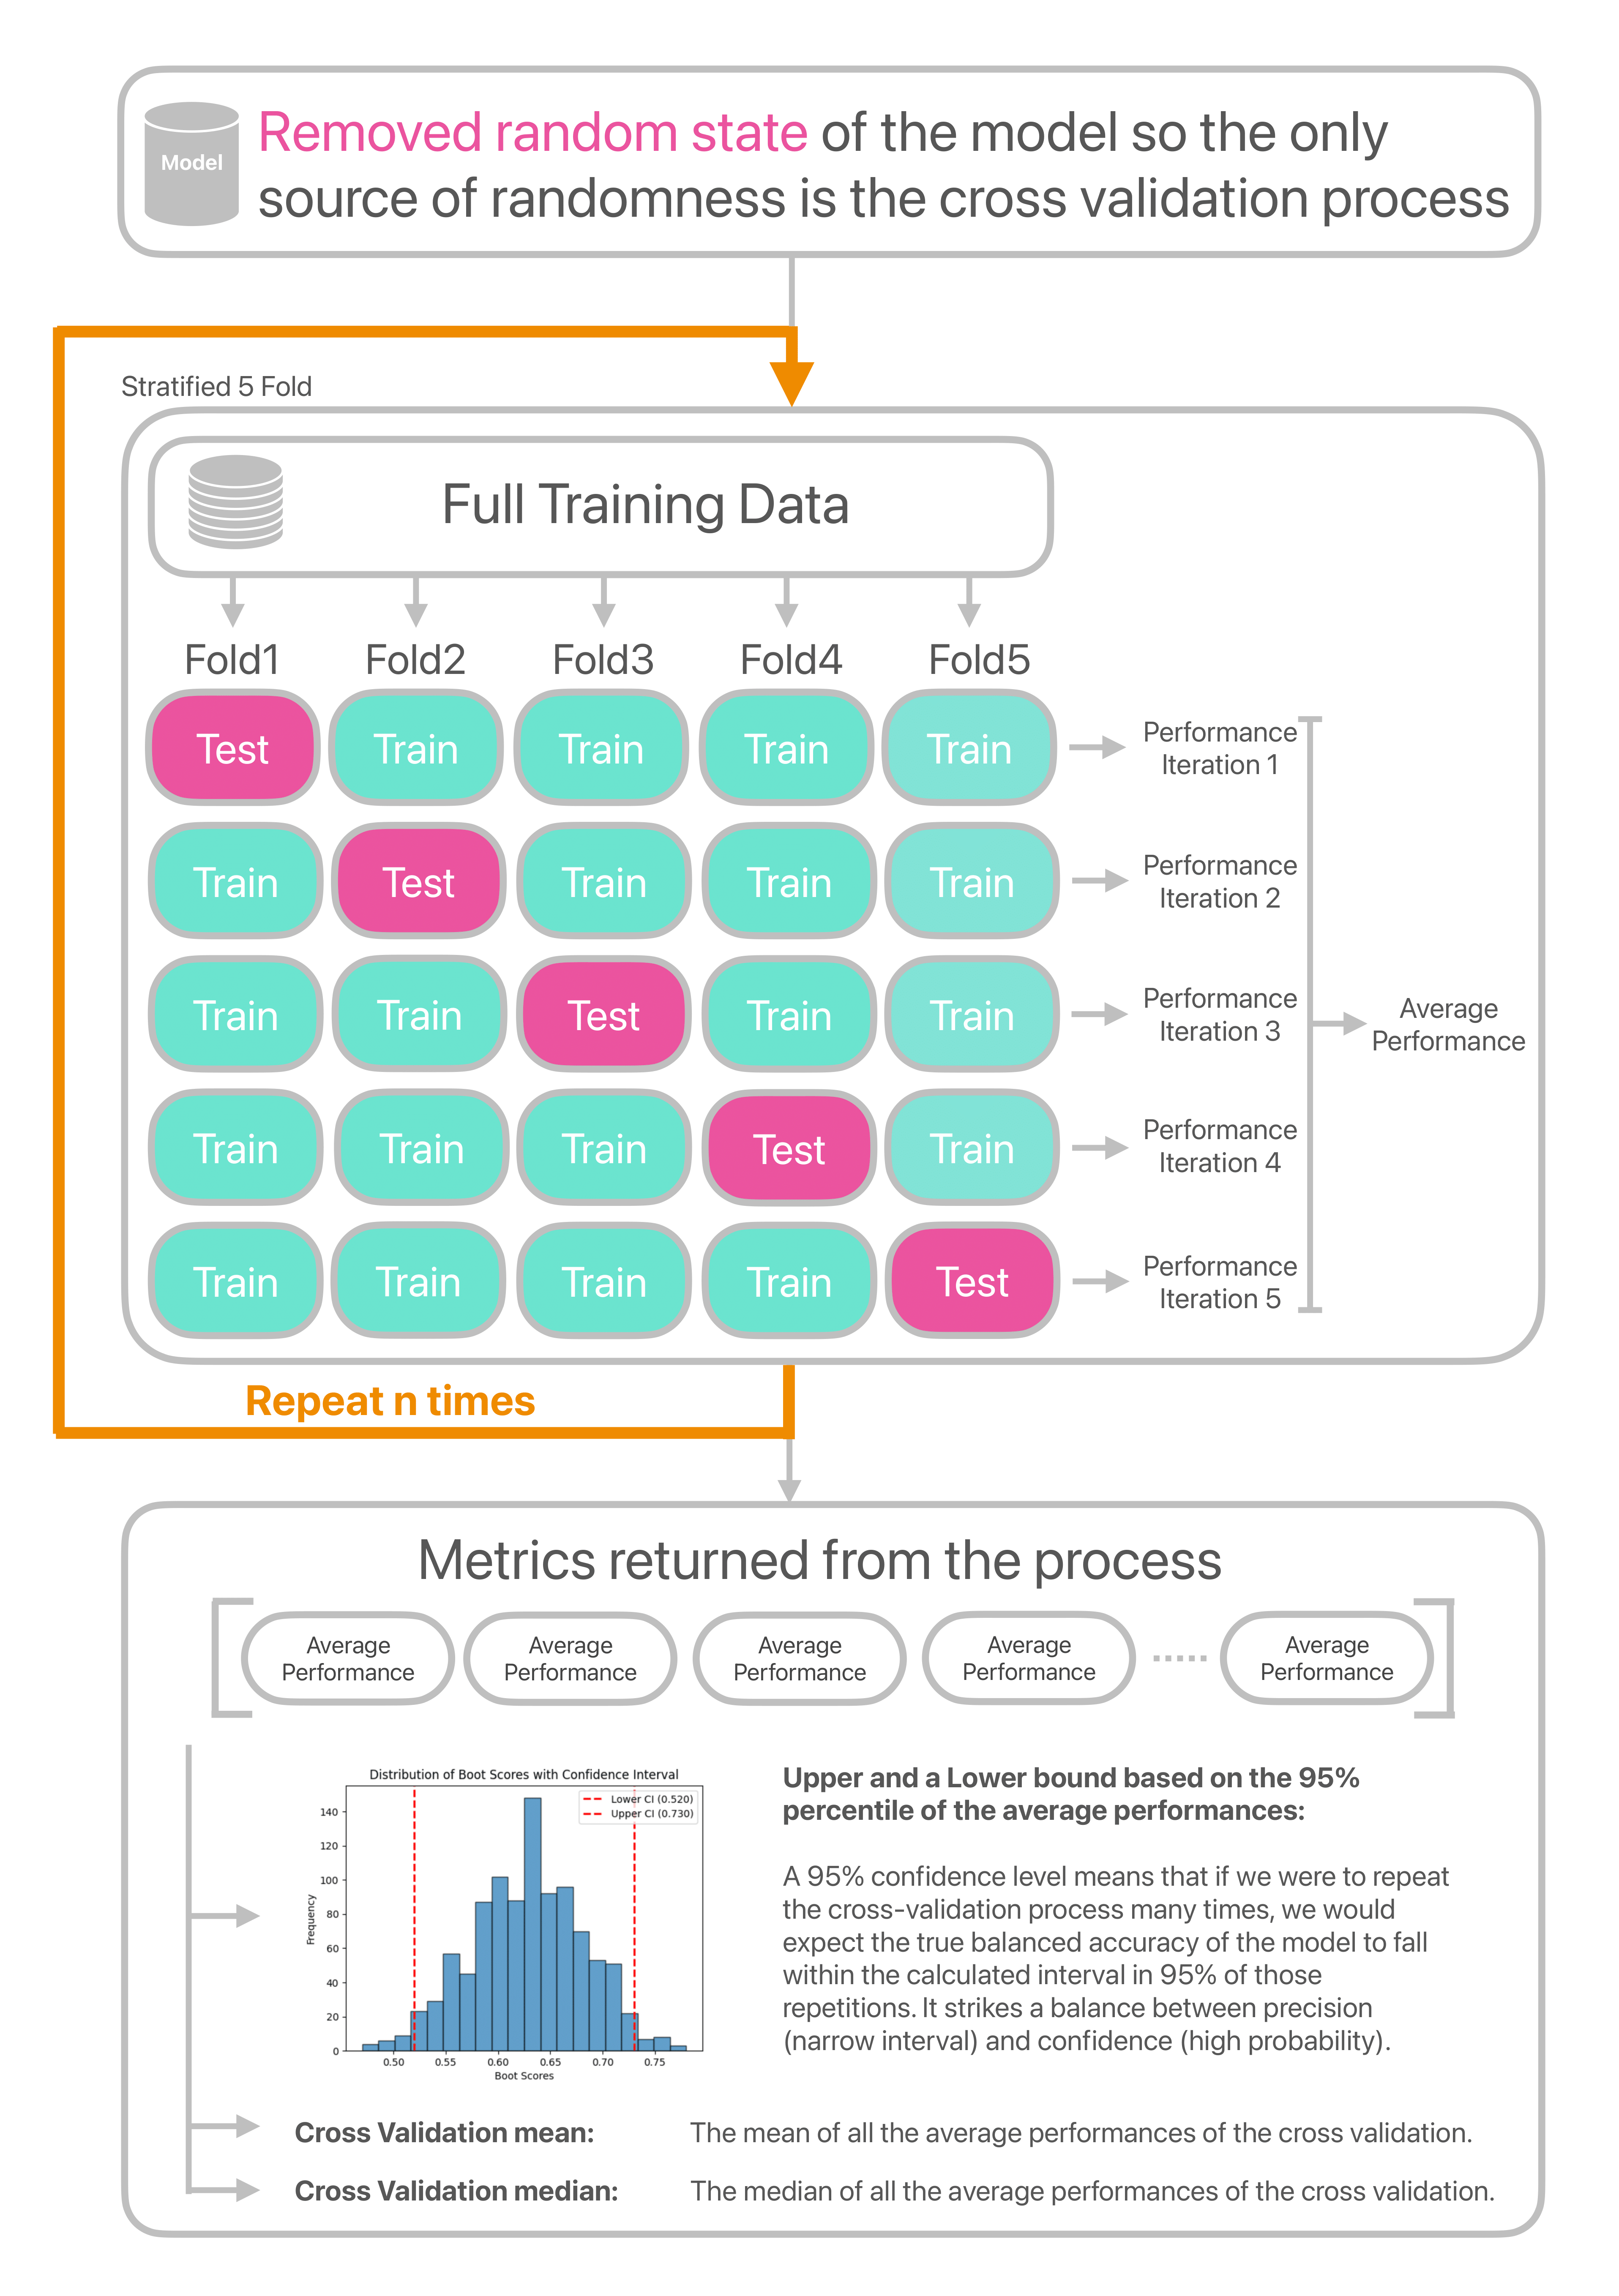
\includegraphics[width=0.9\textwidth]{images/Bootstrapping-1.png}
  \caption[Confidence interval estimation diagram using repeated stratified 5-fold cross-validation]{This diagram illustrates the process of estimating the confidence interval of a model's performance using repeated stratified k-fold cross-validation. Initially, the model's random state is removed to ensure the cross-validation process is the sole source of randomness. Stratified k-fold cross-validation (k=5) is used to evaluate model performance, with the average score across folds representing a single iteration's result. This entire cross-validation procedure is repeated 'n' times (e.g., 1000) to simulate the variability in performance across different random splits. The resulting 'n' average performance scores are then used to calculate the confidence interval. These bounds indicate the range within which we expect the model's true performance to lie with a high degree of confidence, providing a robust measure of the model's reliability.}
  \label{fig:Bootstrapping-1}
\end{figure}

\begin{figure}[H]
  \centering
  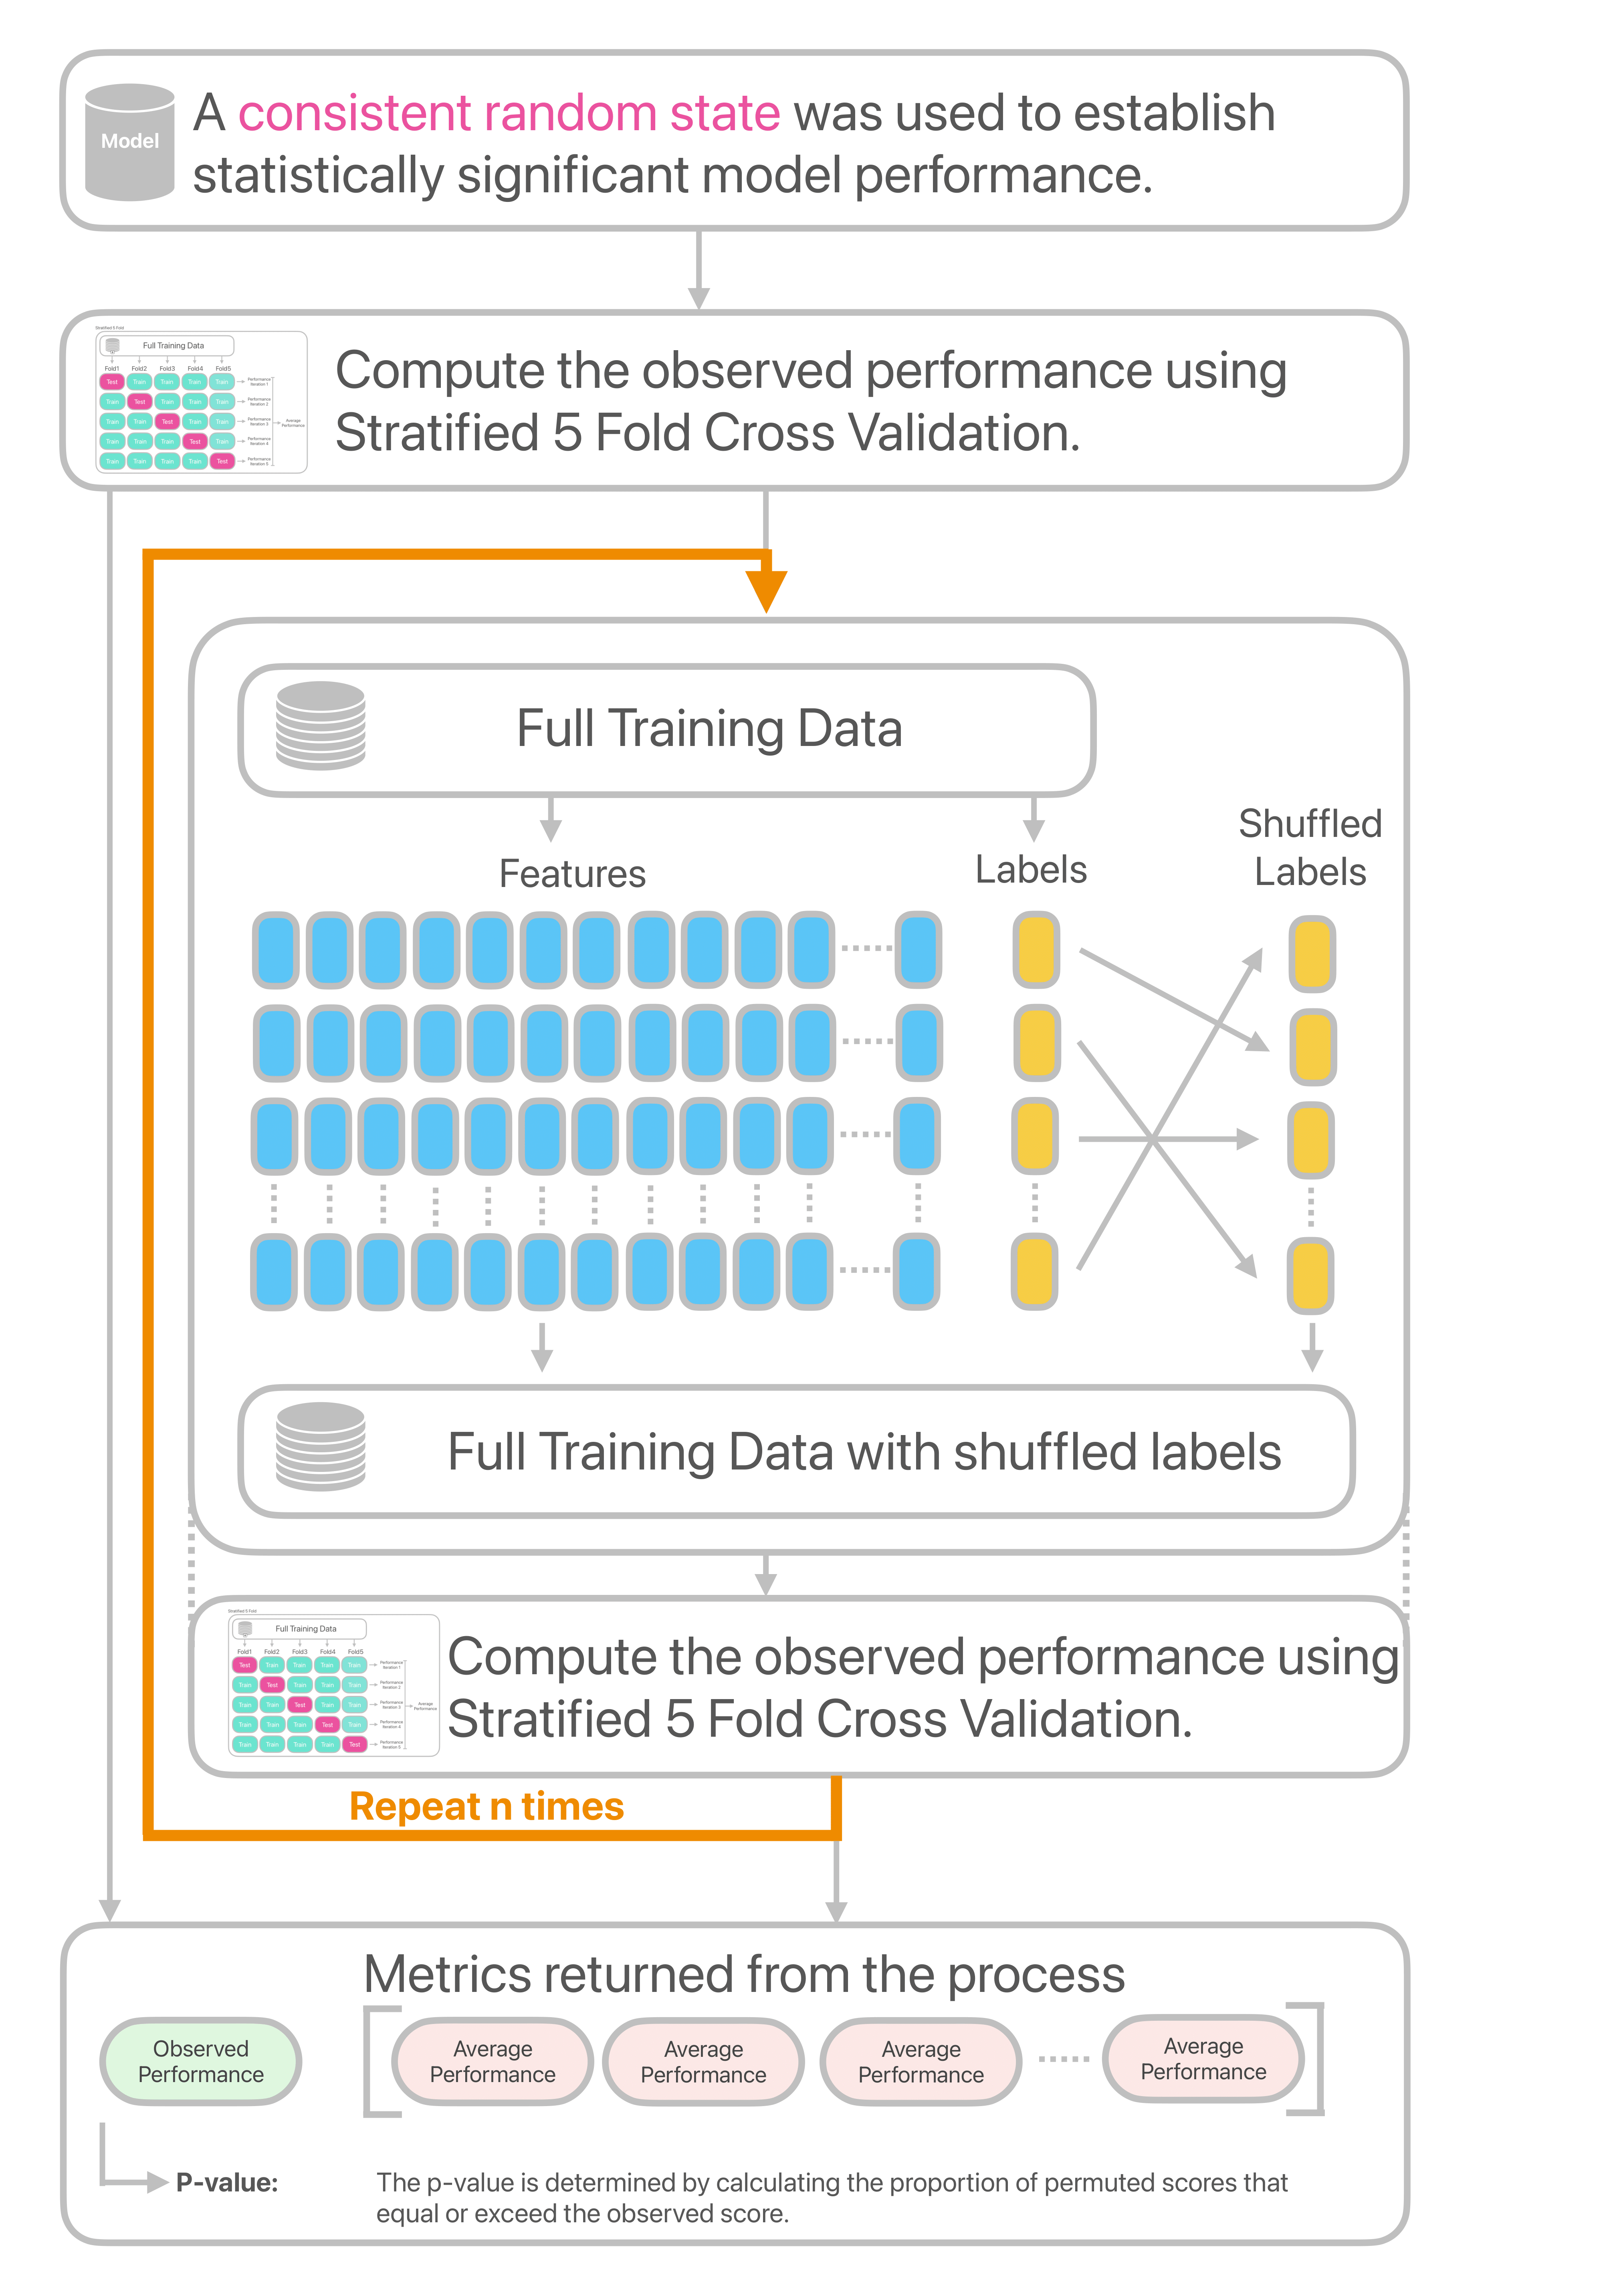
\includegraphics[width=0.9\textwidth]{images/P-value_test-1.png}
  \caption[Evaluating model significance via permutation testing and p-value calculation diagram]{This diagram illustrates a permutation test designed to evaluate the statistical significance of a model's performance. Initially, a consistent random state is set to ensure reproducible results. The model's performance is first assessed on the original data using stratified 5-fold cross-validation, yielding the 'observed performance.' Subsequently, to determine if this performance is merely due to chance, the labels are repeatedly shuffled. For each shuffled dataset, the model's performance is re-evaluated using the same stratified 5-fold cross-validation. This process is repeated 'n' times, resulting in a distribution of 'permuted performances.' Finally, the p-value is calculated as the proportion of permuted performances that equal or exceed the observed performance, indicating the likelihood of obtaining such performance by chance alone.}
  \label{fig:P-value_test-1}
\end{figure}


\subsection{Findings for Consensus model}
\label{sec:findings_for_consensus_model}
\noindent
A primary observation was the marked heterogeneity in the optimal modeling strategies across the different data types, supporting the core premise of the multi-pipeline approach. When utilizing the original, uncompressed features, the best-performing configurations (selected based on validation set performance, with CV MEAN and p-value as tie breakers), are summarized below:
\begin{table}[H]
    \centering
    \hspace*{-1cm}
    \scalebox{0.8}{%
    \begin{tabular}{l l l l l l l}
        \toprule
        Data Type & Oversampling & Best Model & Train Balanced Acc. & Train $p$-value & Val. F1 & Val. Balanced Acc. \\
        \midrule
        cytokines & smote & Logistic Regression & 0.712 & 0.010 & 0.815 & 0.750 \\
        cytometry & smote & Logistic Regression & 0.724 & 0.045 & 0.815 & 0.750 \\
        clonal breadth & random & Naive Bayes & 0.655 & 0.099 & 0.500 & 0.667 \\
        clonal depth & smote & Decision Tree & 0.559 & 0.154 & 0.767 & 0.833 \\
        RNA & smote & Random Forest & 0.810 & 0.000 & 0.514 & 0.500 \\
        \bottomrule
    \end{tabular}}
    \caption[Optimal Modeling Configurations Uncompressed Features]{Optimal Modeling Configurations for Uncompressed Features}
    \label{tab:optimal_configs_uncompressed}
\end{table}

\noindent
The best-performing model for each data type generated the following predictions on their respective test sets: for cytokines, the prediction was $[1\ 1\ 1\ 0\ 0\ 0]$ with a test accuracy of 0.333; for cytometry, the prediction was $[1\ 0\ 0\ 0\ 0\ 0]$ with a test accuracy of 0.667; for clonal breadth, the prediction was $[1\ 0\ 0\ 1\ 0\ 0]$ with a test accuracy of 0.500; for clonal depth, the prediction was $[0\ 0\ 0\ 0\ 1\ 0]$ with a test accuracy of 1.0; and for RNA, the prediction was $[0\ 1\ 0\ 0\ 1\ 0]$ with a test accuracy of 0.833.\\
\\
A consensus prediction was derived by applying majority voting across these individual model outputs, resulting in a final prediction of $[1\ 0\ 0\ 0\ 0\ 0]$. This consensus prediction was then evaluated against the true labels which were $[0\ 0\ 0\ 0\ 1\ 0]$.\\
\\
The overall performance of the consensus prediction on the test set yielded an accuracy of 0.667 and a balanced accuracy of 0.400. A more detailed breakdown of the consensus performance is provided by the classification report:
\begin{table}[h!]
    \centering
    \begin{tabular}{l c c c c}
        \toprule
        Class & Precision & Recall & F1-Score & Support \\
        \midrule
        0 & 0.80 & 0.80 & 0.80 & 5 \\
        1 & 0.00 & 0.00 & 0.00 & 1 \\
        \midrule
        Accuracy &       &      & 0.67 & 6 \\
        Macro Avg & 0.40 & 0.40 & 0.40 & 6 \\
        Weighted Avg & 0.67 & 0.67 & 0.67 & 6 \\
        \bottomrule
    \end{tabular}
    \caption[Consensus Classification Report Uncompressed Features]{Consensus Classification Report for Uncompressed Features}
    \label{tab:consensus_report_uncompressed}
\end{table}

\noindent
Further investigation involved applying PCA-based feature compression within each pipeline. This led to a different set of optimal configurations:
\begin{table}[H]
    \centering
    \hspace*{-1cm}
    \scalebox{0.8}{%
    \begin{tabular}{l l l l l l l}
        \toprule
        Data Type & Oversampling & Best Model & Train Balanced Acc. & Train $p$-value & Val. F1 & Val. Balanced Acc. \\
        \midrule
        cytokines & random & Naive Bayes & 0.630 & 0.076 & 0.815 & 0.750 \\
        cytometry & smote & Decision Tree & 0.725 & 0.009 & 0.815 & 0.750 \\
        clonal breadth & random & Naive Bayes & 0.655 & 0.099 & 0.500 & 0.667 \\
        clonal depth & smote & Decision Tree & 0.559 & 0.154 & 0.767 & 0.833 \\
        RNA & smote & Logistic Regression & 0.789 & 0.011 & 0.667 & 0.625 \\
        \bottomrule
    \end{tabular}}
    \caption[Optimal Modeling Configurations Compressed Features]{Optimal Modeling Configurations for Compressed Features}
    \label{tab:optimal_configs_compressed}
\end{table}
\noindent
The best-performing model for each data type generated the following predictions on their respective test sets: for cytokines, the prediction was $[0\ 0\ 0\ 0\ 0\ 0]$ with a test accuracy of 0.833; for cytometry, the prediction was $[1\ 0\ 0\ 0\ 0\ 0]$ with a test accuracy of 0.667; for clonal breadth, the prediction was $[1\ 0\ 0\ 1\ 0\ 0]$ with a test accuracy of 0.500; for clonal depth, the prediction was $[0\ 0\ 0\ 0\ 1\ 0]$ with a test accuracy of 1.0; and for RNA, the prediction was $[0\ 1\ 0\ 0\ 0\ 0]$ with a test accuracy of 0.667.\\
\\
A consensus prediction was derived by applying majority voting across these individual model outputs, resulting in a final prediction of $[0\ 0\ 0\ 0\ 0\ 0]$. This consensus prediction was then evaluated against the true labels which were $[0\ 0\ 0\ 0\ 1\ 0]$.\\
\\
The overall performance of the consensus prediction on the test set yielded an accuracy of 0.833 and a balanced accuracy of 0.500. A more detailed breakdown of the consensus performance is provided by the classification report:
\begin{table}[h!]
    \centering
    \begin{tabular}{l c c c c}
        \toprule
        Class & Precision & Recall & F1-Score & Support \\
        \midrule
        0 & 0.83 & 1.00 & 0.91 & 5 \\
        1 & 0.00 & 0.00 & 0.00 & 1 \\
        \midrule
        Accuracy &       &      & 0.83 & 6 \\
        Macro Avg & 0.42 & 0.50 & 0.45 & 6 \\
        Weighted Avg & 0.69 & 0.83 & 0.76 & 6 \\
        \bottomrule
    \end{tabular}
    \caption[Consensus Classification Report Compressed Features]{Consensus Classification Report for Compressed Features}
    \label{tab:consensus_report_compressed}
\end{table}

\noindent
The consensus prediction based on majority voting of individual data-type specific models trained on the original, uncompressed features achieved an accuracy of 0.667 and a balanced accuracy of 0.400 on the test set.\\
\\
Applying PCA-based feature compression within each pipeline resulted in a different set of optimal configurations for some data types. The consensus prediction from these models, evaluated on the test set, showed an accuracy of 0.833 and a balanced accuracy of 0.500. These results indicate that for this dataset, the use of compressed features yielded better overall and balanced accuracy in the consensus prediction compared to the uncompressed feature approach.\\
\\
The optimal configurations identified across most data types consistently utilized either SMOTE or random oversampling techniques. This highlights the importance of addressing class imbalance to optimize the performance of the individual models. Oversampling likely helped the models to better capture the characteristics of the minority class, mitigating the tendency to predominantly predict the majority class.\\
\\
Several limitations should be acknowledged when interpreting The findings presented so far. The most significant constraint is the very small size of the test set ($n=6$), which severely limits the statistical power of the performance metrics and the generalizability of the results. The precision of an estimate of the performance outside the sample is heavily dependent on the absolute size of the validation or test set ($n$). This relationship is quantitatively expressed by the formula for the standard error of the measured accuracy: $\sqrt{p(1-p)/n}$, where $p$ is the true accuracy. A smaller standard error indicates that the measured accuracy is likely closer to the true accuracy.\\
\\
For a test set size of $n=6$, the uncertainty is substantial. Using the formula, the standard error is largest when $p=0.5$, resulting in a standard error of $\sqrt{0.5 \times 0.5 / 6} = \sqrt{0.25 / 6} \approx \sqrt{0.0417} \approx 0.204$. This translates to a standard error of roughly 20.4\%. Even at higher accuracies, such as $p=0.8$, the standard error remains considerably large: $\sqrt{0.8 \times 0.2 / 6} = \sqrt{0.16 / 6} \approx \sqrt{0.0267} \approx 0.163$, or about 16.3\%.\\
\\
This magnitude of standard error implies that any accuracy value calculated on this 6-sample test set is a very imprecise estimate of the model's true performance. If, for instance, the model achieved an accuracy of 0.667 (4 out of 6 correct), the true accuracy could plausibly be significantly higher or lower purely due to random chance in the selection of these 6 samples. Similarly, an accuracy of 0.833 (5 out of 6 correct) also carries a large margin of error. This contrasts sharply with scenarios requiring validation sets in the hundreds of thousands to achieve very small standard errors (e.g., 0.1\% or 1\%).\\
\\
Looking at this from another perspective, the small sample size directly impacts the width of confidence intervals, such as the Clopper-Pearson interval, which is commonly used for proportions based on small sample sizes. The Clopper-Pearson interval provides a range of plausible values for the true population proportion (accuracy in this case) based on the observed sample proportion. While the Clopper-Pearson method is based on binomial probabilities rather than a simple formula involving standard error, it is fundamentally driven by the same underlying sampling variability. Increasing the sample size ($n$) reduces this variability, leading to a smaller standard error and, consequently, a narrower Clopper-Pearson confidence interval. For our test set of $n=6$, the resulting confidence intervals for the observed accuracies are very wide. For an observed accuracy of 0.667 (4/6), the 95\% Clopper-Pearson confidence interval is approximately $[0.299, 0.925]$, a width of about 0.626. For an observed accuracy of 0.833 (5/6), the 95\% confidence interval is approximately $[0.359, 0.996]$, a width of about 0.637. This shows that even with a measured accuracy of 0.833, the true accuracy could plausibly be as low as around 36\% due to the limited sample size.\\
\\
Given that simple majority voting did not produce exceptional consensus results, further exploration of more sophisticated ensemble aggregation methods was not pursued in this study. Future work could investigate techniques such as weighted voting (where individual model contributions are weighted based on factors like validation performance or modality relevance), stacking (employing a meta-learner to combine predictions), or rank aggregation, which may potentially lead to more robust and balanced consensus predictions.




%\section{SMOTE-Driven Oversampling and SHAP-Based Feature Interpretation Approach}
\section{Feature Identification Methodology}
\todo{In progress...}
\noindent
Given the constraints imposed by the limited dataset ($N=40$), particularly the small number of samples available for independent testing, a primary objective of this study was to explore and identify potentially important features associated with the vaccine response. Standard approaches for model selection and rigorous performance evaluation typically rely on larger validation or test sets to provide reliable estimates of out-of-sample performance and prevent overfitting during the selection process. However, as discussed in the previous section, the extremely small size of our test set ($n=6$) introduces substantial uncertainty into any performance metric, as demonstrated by the large standard errors and wide Clopper-Pearson confidence intervals. While a test set size of $n=8$ offers a marginal improvement in reducing the width of the confidence interval compared to an even smaller sample like $n=6$, it still leaves a significant degree of uncertainty, rendering traditional rigorous model selection based on distinct validation/test splits highly problematic and potentially less informative than desired.\\
\\
Recognizing these severe data limitations, my approach to feature identification prioritizes exploration and hypothesis generation. I trained a variety of models across different data types, incorporating various SMOTE (Synthetic Minority Over-sampling Technique) oversampling variations to address the inherent class imbalance in the dataset. To understand the contribution of individual features within these models, I utilized SHAP (SHapley Additive exPlanations \cite{ApprouchForModelPredictions}) values. It is a technique that explains the output of machine learning models by assigning each feature an importance value based on its contribution to the model’s predictions using game theory.

\subsection{Pipeline Structure for Heterogeneous Datasets}
To systematically implement the exploratory strategy outlined above a standardized computational pipeline was employed (very similar to the pipeline in Section~\ref{sec:consensus_model_approach}). This pipeline, visually detailed in Figure~\ref{fig:pipeline-2}, ensures consistency in data handling, model training, and the generation of performance metrics across all experimental conditions. It encompasses crucial steps from initial data preprocessing and targeted oversampling of the training data to model fitting and the assessment of performance on the hold-out test set. The models generated and evaluated through this workflow form the basis for the subsequent performance filtering and aggregation of SHAP values aimed at identifying potentially important features. The following sections describe each stage of this pipeline.

\subsubsection{Preprocessing \hyperref[fig:pipeline-2]{(A, B, C, F)}}
\noindent The initial data preparation steps, specifically handling missing data \hyperref[fig:pipeline-2]{(A)}, compressing correlated features \hyperref[fig:pipeline-2]{(B)}, and encoding class labels \hyperref[fig:pipeline-2]{(C)}, and later scaling the features \hyperref[fig:pipeline-2]{(F)}, were performed using the identical procedures as detailed in Section~\ref{sec:consensus_model_approach}.


\pagebreak
\begin{figure}[H]
  \centering
  \hspace*{-0.9cm} % Adjust spacing as needed
  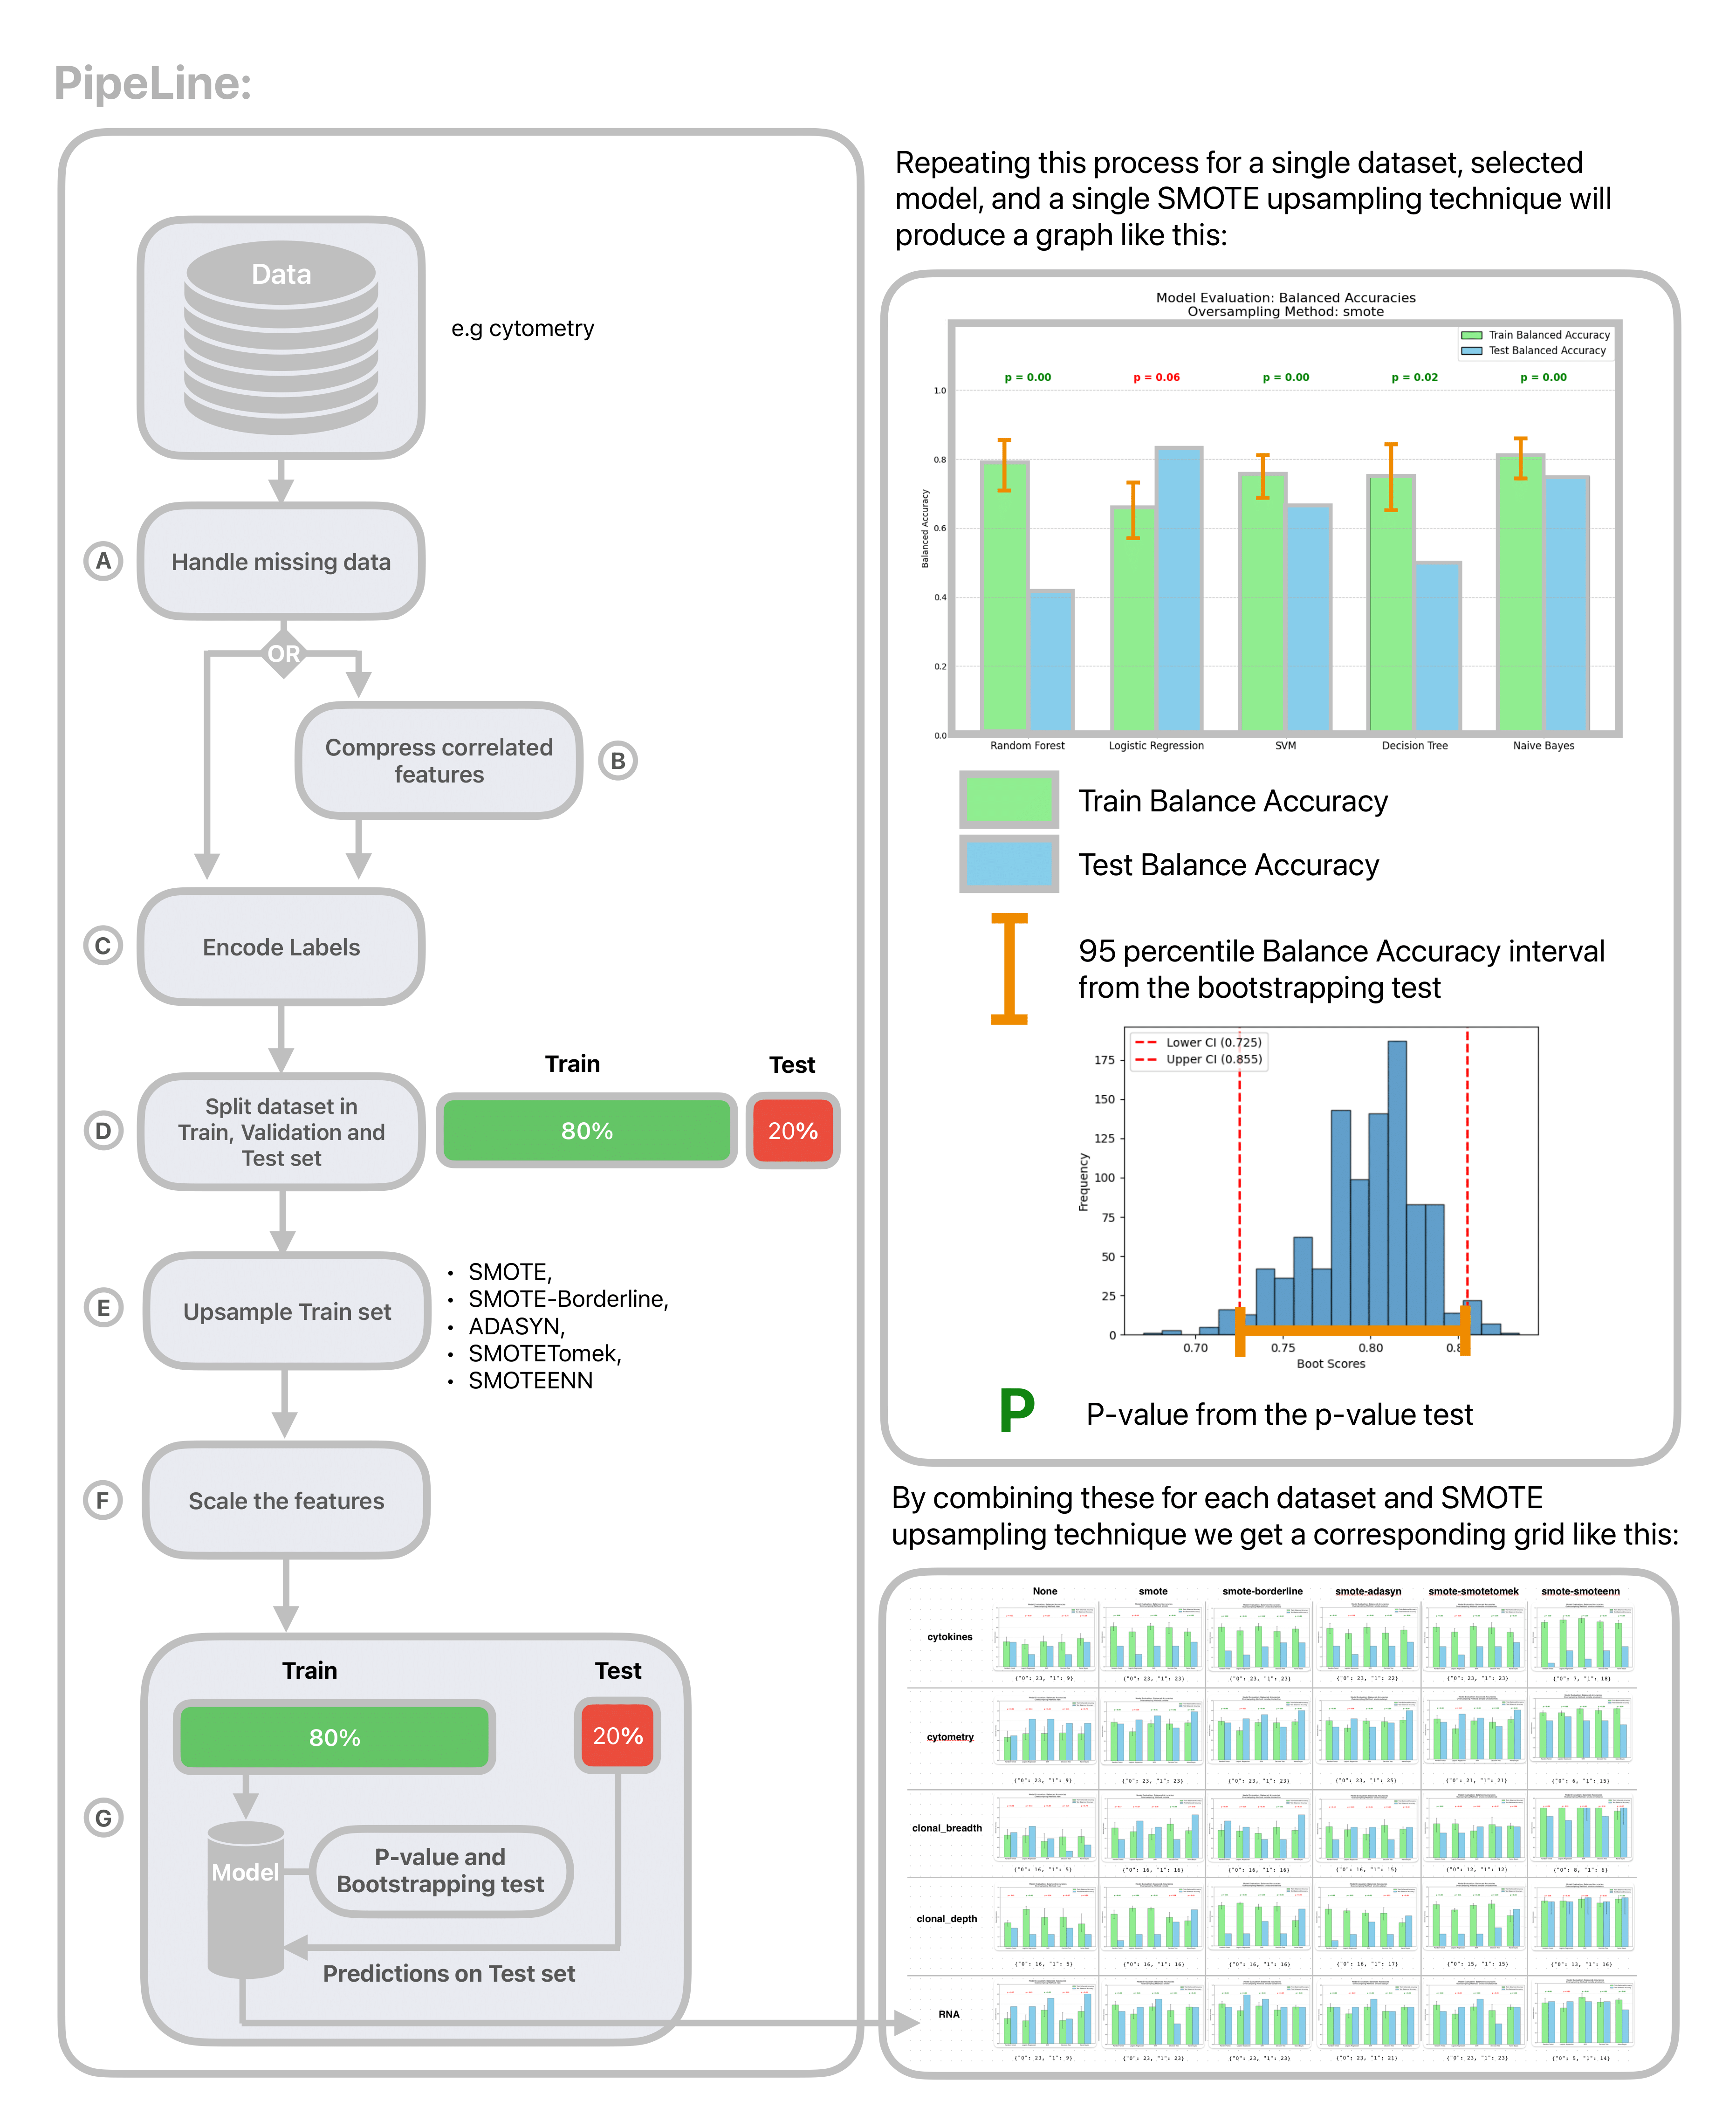
\includegraphics[width=1.1\textwidth]{images/Pipeline-2.png} % Ensure path is correct
  \caption[Feature Identification models pipeline diagram]{ The diagram illustrates the multi-model pipeline used for constructing the models.  Each individual model follows a standardized preprocessing workflow: data loading, preprocessing (A: Missing data handling, B: Feature compression, C: Label encoding, F: Feature scaling), data splitting (D), training set oversampling using various SMOTE techniques (E), model training, and evaluation (G). Performance on train and test sets is measured by Balanced Accuracy, with 95\% bootstrap confidence intervals and p-value testing, repeated across datasets and SMOTE methods as illustrated.}
  \label{fig:pipeline-2}
\end{figure}

\subsubsection*{Split dataset \hyperref[fig:pipeline-2]{(D)}}
As mentioned earlier, due to the extreme data scarcity ($N=40$), the decision was made to partition the data into a training set comprising of 80\% of the samples ($n=32$) and a hold-out test set containing the remaining 20\% ($n=8$). Further splitting the training data to create a separate validation set would drastically reduce the number of samples available for model training, likely impairing the models' ability to learn meaningful patterns from the data. Furthermore, dividing the test set further would make the individual subsets too small to yield any statistically stable or meaningful performance estimates as discussed in the previous Section~\ref{sec:findings_for_consensus_model}. Therefore, I made the pragmatic decision to use the performance observed \textit{only} on the hold-out test set ($n=8$) as a preliminary criterion for filtering models whose SHAP explanations would be further analyzed and aggregated.\\
\\
While conventionally using the test set for model selection is strongly discouraged due to the risk of test set overfitting and obtaining overly optimistic performance estimates, the extreme data scarcity in this study necessitates this deviation from standard practice. I utilized the performance on the $n=8$ test set not for precise model ranking or performance reporting, but primarily as a coarse filter: models that perform poorly even on this small test set are excluded, as their low scores, despite the uncertainty, suggest they are unlikely to generalize well. Conversely, models that achieve higher scores on this $n=8$ test set are retained. While the uncertainty on an $n=8$ sample means that a high score does not guarantee good true performance, these models still possess the potential to be good performers. Excluding them based on the high variance associated with the $n=8$ estimate would be overly conservative and might discard promising candidates for feature analysis. This approach is used with the explicit understanding that it is a pragmatic compromise driven by data constraints. The subsequent findings regarding feature importance derived from aggregating SHAP values of these filtered models are to be interpreted strictly as exploratory hypotheses rather than definitive conclusions. The goal is to identify features that appear consistently important across models that show some minimal indication of potential relevance on the limited unseen data, providing potential candidates for validation in future studies with larger datasets.

\subsubsection*{Up-sample Train set \hyperref[fig:pipeline-2]{(E)}}
It became evident that strategies involving data upsampling, such as random oversampling and particularly SMOTE, played a crucial role in improving model performance when dealing with small, imbalanced datasets. Motivated by these findings, I extended the analysis to investigate several variations of SMOTE. These methods aim to address class imbalance more effectively than standard SMOTE by refining the process of generating synthetic samples or combining it with data cleaning techniques, thereby allowing models to extract more useful patterns and generalize better from sparse data.\\
\\
The first method used was standard SMOTE \cite{Chawla2002SMOTE}, which, as previously detailed in Subsection~\ref{subsec:pipeline_structure_for_heterogeneous_datasets} (Up-sample Train set), synthesizes new minority instances by generating samples along the lines connecting existing minority samples and their selected k-nearest minority neighbors (illustrated conceptually in Figure~\ref{fig:SMOTE_explained}). Standard SMOTE, while a foundational technique, has known weaknesses, as detailed in Subsection~\ref{subsec:pipeline_structure_for_heterogeneous_datasets} and conceptually illustrated in Figure~\ref{fig:SMOTE_weaknesses}. The variations of SMOTE included in this study were developed to mitigate these issues, either by focusing synthetic sample generation on more informative areas or by combining oversampling with data cleaning steps.\\
\begin{figure}[h!]
  \centering
  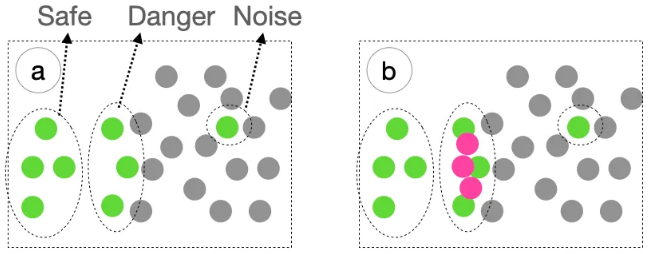
\includegraphics[width=0.9\textwidth]{images/SMOTE-Borderline.png}
  \caption[Illustration of Borderline-SMOTE Sample Generation]{Illustration of the Borderline-SMOTE synthetic sample generation process. Panel (a) shows minority class samples (green) categorized into 'Safe', 'Danger' (borderline), and 'Noise' zones based on the ratio of majority class neighbors (grey) among their k-nearest neighbors. Panel (b) demonstrates how synthetic minority samples (pink) are generated specifically in the 'Danger' zone. Figure adapted from figure 9 presented in \cite{Truong2022SMOTEVariants}.}
  \label{fig:SMOTE-Borderline}
\end{figure}
\\
\noindent
As a prime example of a variation focusing on challenging areas, Borderline-SMOTE \cite{Han2005Borderline} was applied. Proposed by Han et al. in 2005, this variant is based on the reasoning that minority samples located in the borderline regions near the decision boundary are particularly difficult for classifiers to learn. By specifically adding more synthetic samples in these ambiguous regions, the method aims to help the classifier distinguish between classes better. The core idea of Borderline-SMOTE is to first identify minority samples that are in 'danger' of being misclassified. Using k-nearest neighbors (KNN), each minority sample is classified into a 'noise', 'safe' or 'danger' zone based on the ratio ($r$) of majority instances among its neighbors. A sample is considered 'noise' if all its neighbors are majority class ($r=1$), in a 'safe' zone if most neighbors are minority class ($r < 0.5$), and in the 'danger' (or 'borderline') zone if the mix is significant ($0.5 \leq r < 1$). Unlike standard SMOTE which oversamples all minority samples, Borderline-SMOTE focuses its synthetic sample generation only on those minority samples identified as being in the 'danger' zone, synthesizing new instances by interpolating between a danger-zone sample and its minority neighbors. This targeted approach aims to reinforce the decision boundary in regions considered critical for classification, as illustrated in Figure~\ref{fig:SMOTE-Borderline}.\\
\begin{figure}[h!]
  \centering
  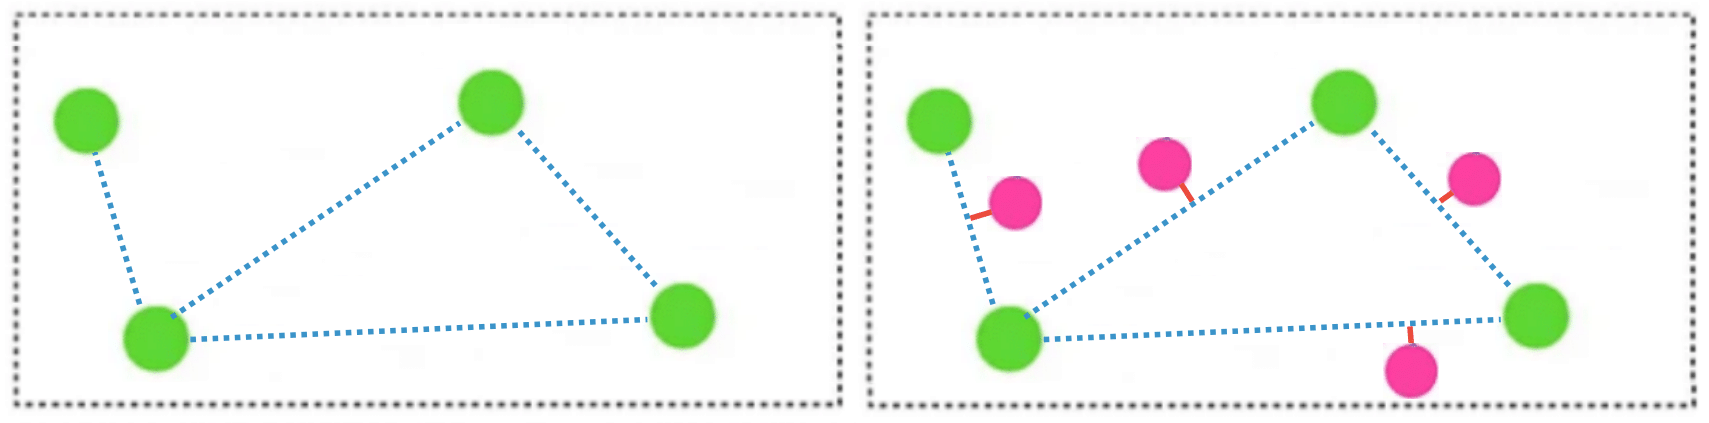
\includegraphics[width=0.9\textwidth]{images/SMOTE-ADASYN.png}
  \caption[Illustration of ADASYN Sample Generation]{Illustration of the ADASYN synthetic sample generation process. The left panel shows original minority samples. The right panel shows synthetic minority samples (pink) generated by ADASYN, demonstrating the addition of small random variations that cause the synthetic points to be slightly scattered around the interpolation lines between neighbors. Figure made in same style as images presented in \cite{Truong2022SMOTEVariants}.}
  \label{fig:SMOTE-ADASYN}
\end{figure}
\\
\noindent
Another approach included was ADASYN (Adaptive Synthetic Sampling) \cite{He2008ADASYN}. Presented as an improved version of standard SMOTE, ADASYN incorporates a modification to the synthetic sample generation process. After creating synthetic points via interpolation similar to SMOTE, ADASYN adds small random values $\lambda \in [0, 1]$ to these generated points. This addition introduces a degree of variance, resulting in synthetic samples that are slightly scattered around the interpolating line rather than being strictly linearly correlated with the original samples, as illustrated in Figure~\ref{fig:SMOTE-ADASYN}. This aims to make the generated data distribution more realistic and potentially help models generalize better.\\
\begin{figure}[h!]
  \centering
  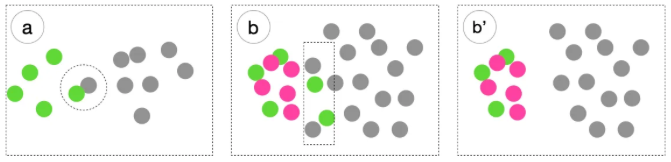
\includegraphics[width=0.9\textwidth]{images/SMOTE-Tomek.png}
  \caption[Illustration of SMOTE-Tomek Process]{Illustration of the SMOTE-Tomek process. Panel (a) conceptually shows a Tomek link, defined as a pair of instances from different classes that are mutual nearest neighbors. Panel (b) depicts a dataset after standard SMOTE oversampling, including original (green and grey) and synthetic (pink) samples. Panel (b') shows the result after the removal of Tomek links, which helps to clean the decision boundary by eliminating ambiguous points near the interface between classes. Figure adapted from figure 5 presented in \cite{Truong2022SMOTEVariants}.}
  \label{fig:SMOTE-Tomek} % Corrected label spelling
\end{figure}
\\
\noindent
Furthermore, hybrid techniques combining SMOTE oversampling with data cleaning were also included in the analysis pipeline. SMOTE-Tomek \cite{Batista2004Study} implements a two-stage process. It first applies standard SMOTE to oversample the minority class, and then utilizes the concept of Tomek links to perform a cleaning step. A Tomek link is defined as a pair of instances $(x_i, x_j)$ from different classes that are mutual closest neighbors, meaning $x_i$ is the nearest neighbor of $x_j$, and $x_j$ is the nearest neighbor of $x_i$. As conceptually illustrated in Figure~\ref{fig:SMOTE-Tomek}(a), these pairs often represent ambiguous points located at the borderline between classes, where misclassification is likely to occur. The idea behind the Tomek link removal in SMOTE-Tomek is to make the training dataset cleaner by eliminating these ambiguous points at the borderlines. After the initial SMOTE oversampling, all Tomek links involving either original or newly synthesized samples are identified. Then, one or both instances forming each Tomek link are removed. This removal process helps to eliminate noise and clarify the separation between classes, particularly near the decision boundary, as illustrated in Figure~\ref{fig:SMOTE-Tomek}(b and b').\\
\begin{figure}[h!]
  \centering
  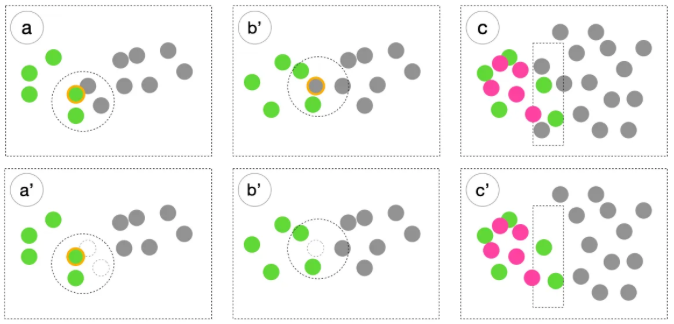
\includegraphics[width=0.9\textwidth]{images/SMOTE-EEN.png}
  \caption[Illustration of SMOTE-ENN Process]{Illustration of the SMOTE-ENN process, focusing on the Edited Nearest Neighbours (ENN) cleaning step. Panels (a) and (a') show an example where a minority sample's (green, highlighted) neighbors are examined, and in (a'), the sample is removed because its class label disagrees with the majority of its k-nearest neighbors. Panels (b) and (b') show a similar example for a majority sample (grey, highlighted) that is removed in (b') based on the same ENN rule. Panels (c) and (c') depict a dataset after SMOTE oversampling (original green/grey, synthetic pink) in (c'), samples inconsistent with their local neighborhood majority, as determined by the ENN rule, have been removed. This cleaning step helps to eliminate noise and ambiguous points, resulting in more clearly defined class boundaries. Figure adapted from figure 7 presented in \cite{Truong2022SMOTEVariants}.}
  \label{fig:SMOTE-ENN} % Corrected label spelling
\end{figure}
\\
\noindent
Similarly, SMOTE-ENN (Edited Nearest Neighbours) \cite{Batista2004Study} is another hybrid technique that follows SMOTE oversampling with a cleaning step based on Wilson’s Edited Nearest Neighbour (ENN) rules. In the ENN component, applied after the initial SMOTE oversampling, the dataset is cleaned based on the local neighborhood consistency of each sample $S_i$. For each sample $S_i$ (which can be original or synthetic), its $k$-nearest neighbors (kNN) are identified, and the ratio ($r$) of majority class instances among these KNN is calculated. The ENN cleaning rule then applies as follows:
\begin{itemize}
    \item If a sample $S_i$ belongs to the minority class and the ratio $r$ of majority instances among its KNN is greater than 0.5 ($r > 0.5$), then the majority instances among its KNN are removed. This scenario is conceptually illustrated in Figure~\ref{fig:SMOTE-ENN}(a and a').
    \item If a sample $S_i$ belongs to the majority class and the ratio $r$ of majority instances among its KNN is less than 0.5 ($r < 0.5$), then the sample $S_i$ itself is removed. This scenario is conceptually illustrated in Figure~\ref{fig:SMOTE-ENN}(b and b').
\end{itemize}
This rule is applied to aggressively clean the dataset by removing instances (original or synthetic) that appear to be mislabeled or that create ambiguity by being inconsistent with their local neighborhood's dominant class. The application of ENN cleaning after SMOTE oversampling results in the removal of inconsistent samples, leading to more clearly defined class clusters, as shown in Figure~\ref{fig:SMOTE-ENN}(c and c'). Compared to Tomek link removal, the ENN cleaning process typically removes more samples, potentially resulting in a more significant clarification of boundaries but also carrying a higher risk of removing potentially informative instances near the true decision boundary.\\
\\
By training separate models for each dataset using training data generated by each of these methods (including 'None' for no oversampling), the analysis allowed for a comprehensive exploration of the impact of different imbalance correction strategies on model performance and subsequent feature importance analysis.

\subsubsection*{Train and Evaluate Models \hyperref[fig:pipeline-2]{(G)}}
In this final stage of the pipeline, the various classification models outlined in Table~\ref{tab:ml_models} were trained and subsequently evaluated. For each dataset and each applied oversampling strategy (including the 'None' case), instances of these models were trained using the respective preprocessed training data partition ($n=32$). Following training, each model's performance was assessed on the untouched hold-out test set ($n=8$).\\
\\
Given the inherent class imbalance of the dataset, Balanced Accuracy was selected as the primary performance metric for evaluating the models in this study, providing a more robust measure than standard accuracy by accounting for the performance on both minority and majority classes. To complement the evaluation on the small test set, additional analyses related to model performance characteristics were conducted on the training data. Specifically, 95\% confidence intervals for the Balanced Accuracy were calculated based on a bootstrapping procedure applied to the training data. This bootstrapping technique, used for reasons related to limited data as discussed in Subsection~\ref{subsec:pipeline_structure_for_heterogeneous_datasets}, is illustrated and explained in detail in Figure~\ref{fig:Bootstrapping-1}.\\
\\
Furthermore, statistical significance was assessed using permutation tests applied to the training data. The permutation test technique, also used for reasons related to limited data as discussed in Subsection~\ref{subsec:pipeline_structure_for_heterogeneous_datasets}, is illustrated and explained in detail in Figure~\ref{fig:P-value_test-1}. This involved repeatedly permuting the true class labels of the training data and recalculating the Balanced Accuracy to determine the likelihood of achieving the observed training performance by chance.\\
\\
The Balanced Accuracy score, its 95\% bootstrapped confidence interval, and the p-value from the permutation test were computed for each trained model under every oversampling condition for each dataset. These performance parameters were then saved. these saved evaluation metrics served as the basis for the subsequent filtering and selection of "best" performing model configurations prior to the SHAP analysis for feature importance identification.

\subsection{Feature Importance Assessment using SHAP}
% \todo{
% \begin{itemize}
%     \item \textbf{Introduction and Purpose:} Explain why feature importance is relevant and introduce SHAP as the chosen method, highlighting its advantages and what SHAP values represent.
%     \item \textbf{Rationale for Using SHAP Across Multiple Models:} Explain the reasoning behind using SHAP on multiple models (e.g., robustness) rather than a single model.
%     \item \textbf{Model Selection for SHAP Analysis:} Clearly describe how the performance metrics from the previous evaluation step were used to select the specific models included in the SHAP analysis.
%     \item \textbf{SHAP Calculation Details:} Describe which data instances were used for SHAP calculation and mention the specific SHAP explainer(s) employed.
% \end{itemize}
% }
\noindent
Understanding which factors contribute to a model's prediction is crucial, particularly in complex biological contexts where machine learning is used to uncover insights into underlying mechanisms. In this study, identifying the features that significantly influence the prediction of vaccine response is key to understanding the potential biological or clinical associations involved. Feature importance methods aim to quantify the contribution of each input feature to the model's output.\\
\\
To assess feature importance and provide interpretable explanations for our models, we employed SHAP (SHapley Additive exPlanations) \cite{ApprouchForModelPredictions}. SHAP is a unified framework rooted in cooperative game theory, using Shapley values to attribute the contribution of each feature to the difference between an individual prediction and the average prediction. Formally, the SHAP value of a feature for a specific instance represents the average marginal contribution of that feature's value to the prediction, considering all possible combinations of features. A fundamental property of SHAP values is their additivity, which provides a clear link between feature contributions and the model's output. For any given instance $x$, the SHAP values ($\phi_i$) for all features $i=1, \dots, M$ sum up to the difference between the model's output for that instance, $f(x)$, and the expected base value (average output) over the dataset, $E[f(x)]$. This relationship can be formally expressed as:
$$ f(x) = E[f(x)] + \sum_{i=1}^M \phi_i $$
Here, $E[f(x)]$ represents the base value of the prediction, which is typically the average prediction over the training data or a representative background dataset. The SHAP value $\phi_i$ for feature $i$ quantifies the feature's contribution to pushing the prediction from this base value $E[f(x)]$ to the final output $f(x)$. A feature with a positive SHAP value ($\phi_i > 0$) increases the model's output relative to the base value, while a negative SHAP value ($\phi_i < 0$) decreases it, as illustrated in Figure~\ref{fig:SHAP-individual-explained}. For binary classification models, SHAP values are typically on the log-odds scale.\\
% images based on https://shap.readthedocs.io/en/latest/example_notebooks/overviews/An%20introduction%20to%20explainable%20AI%20with%20Shapley%20values.html
\begin{figure}[h!]
  \centering
  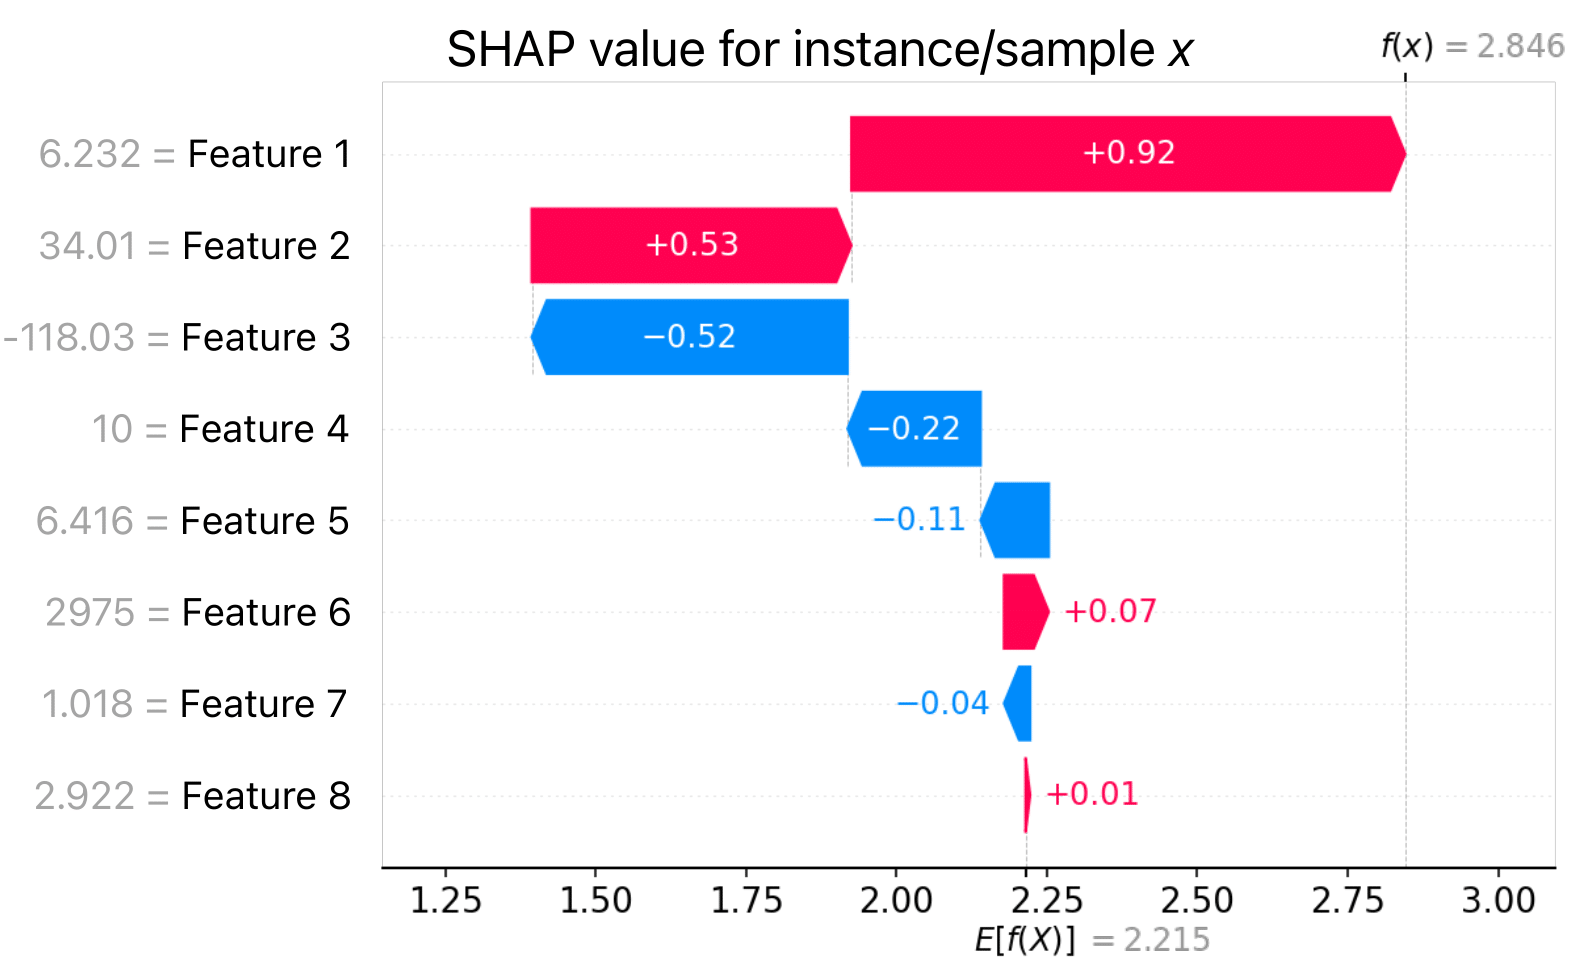
\includegraphics[width=0.9\textwidth]{images/SHAP-explained-individual.png}
  \caption[Example SHAP Individual Explanation Plot]{An example SHAP individual explanation plot for a single instance (sample x). This plot illustrates how each feature's value contributes to the model's prediction for this specific instance, moving from the expected base value ($E[f(x)] = 2.215$) to the final predicted output ($f(x) = 2.846$). Each arrow represents a feature's SHAP value ($\phi_i$); red arrows indicate positive contributions that increase the output, while blue arrows indicate negative contributions that decrease the output. The width of each arrow corresponds to the magnitude of the feature's impact. Features are listed on the left along with their actual values for this instance.}
  \label{fig:SHAP-individual-explained} % Corrected label for clarity
\end{figure}

\begin{figure}[h!]
  \centering
  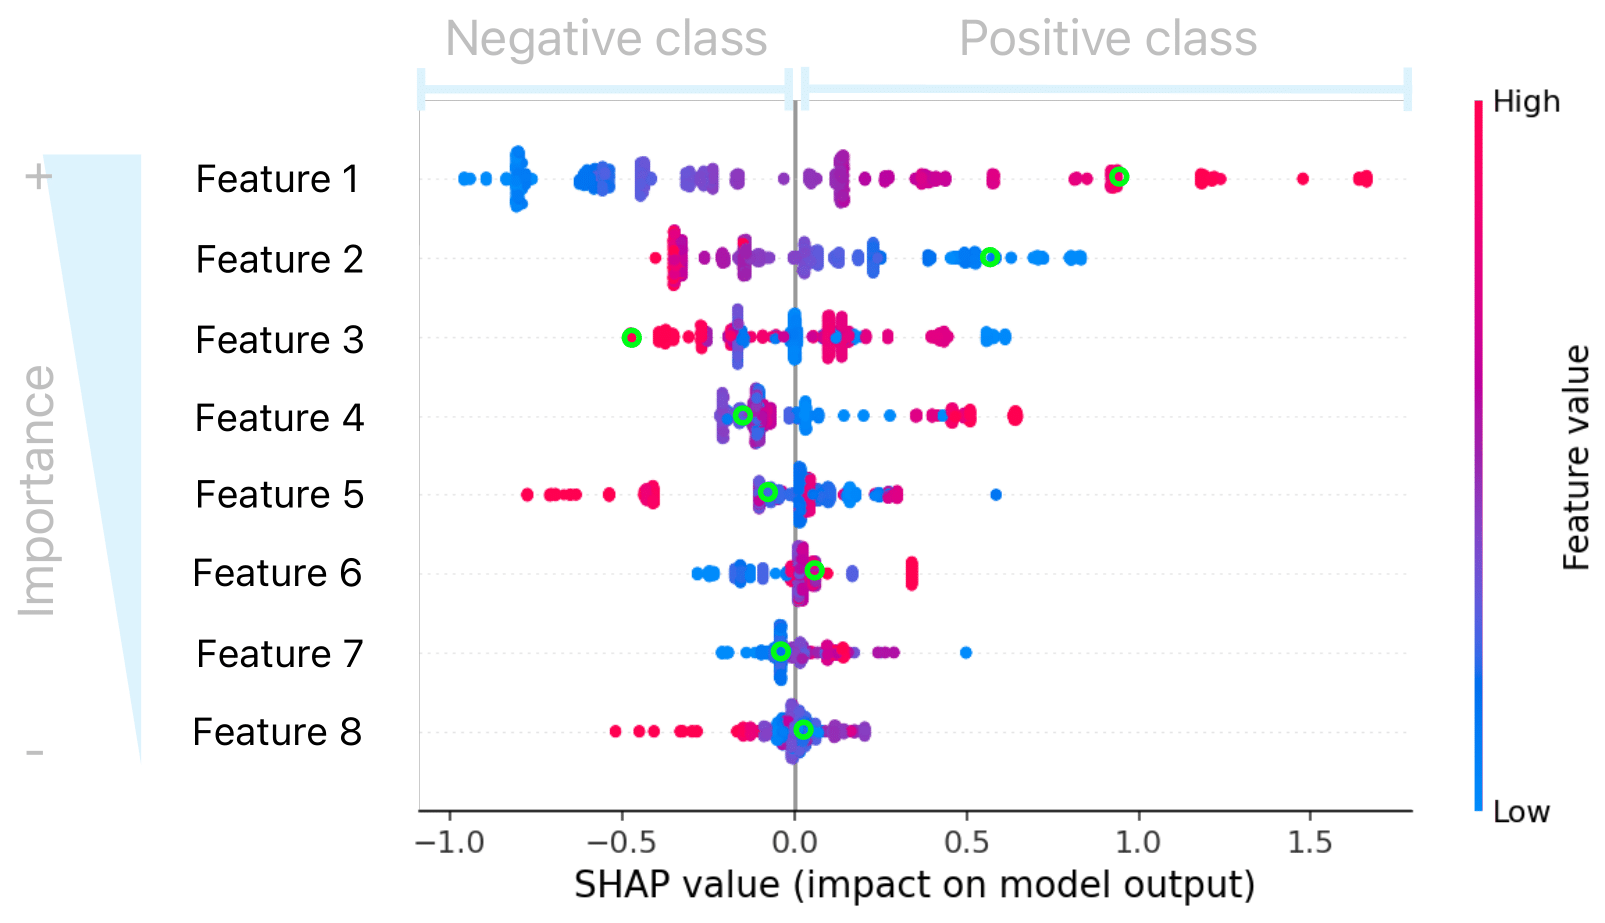
\includegraphics[width=0.9\textwidth]{images/SHAP-explained.png}
  \caption[Example SHAP Summary Plot]{An example SHAP summary plot. This visualization shows the overall importance of features and how their values impact the model's output across a dataset. Features are ranked by importance on the y-axis, the x-axis represents the impact (SHAP value), and the color indicates the feature value (low to high). Points on the left push the prediction towards the negative class, while points on the right push it towards the positive class. Points corresponding to the SHAP values from an individual explanation (as shown in Figure~\ref{fig:SHAP-individual-explained}) are highlighted in green for context.}
  \label{fig:SHAP-plot-explained}
\end{figure}
\noindent
A common and informative visualization of SHAP values across an entire dataset (or a representative subset) is the SHAP summary plot, an example of which is shown in Figure~\ref{fig:SHAP-plot-explained}. This  plot is essentially an aggregation of the individual SHAP explanation plots (like Figure~\ref{fig:SHAP-individual-explained}) for many instances and provides a rich overview of feature importance and the relationship between feature values and their impact on model predictions. Interpreting the SHAP summary plot involves understanding its key components:
\pagebreak
\begin{itemize}
    \item \textbf{Y-axis:} Features are listed on the vertical axis, ordered by their overall importance from top to bottom. A feature's overall importance is typically measured by the average of the absolute SHAP values for that feature across all instances in the plot. Features higher on the list have a greater average impact on the magnitude of the model's output difference from the average prediction.
    \item \textbf{X-axis:} The horizontal axis represents the SHAP value ($\phi_i$) (impact on model output). For a binary classification model trained to predict Label 1 (the positive class) versus Label 0 (the negative class), positive SHAP values ($>0$) indicate that the feature's value increases the model's output, pushing the prediction towards the positive class (Label 1). Conversely, negative SHAP values ($<0$) indicate that the feature's value decreases the model's output, pushing the prediction towards the negative class (Label 0). The position of a point along the x-axis shows the magnitude and direction of a specific feature's impact for a particular instance.
    \item \textbf{Color:} Each point on the plot is colored according to the actual value of the feature it represents for that specific data instance. The color bar shown on the right (as in Figure~\ref{fig:SHAP-plot-explained}), maps the color to the feature value scale (e.g., red indicates a high feature value, and blue indicates a low feature value). This allows for examining how the value of a feature relates to the direction and magnitude of its impact.
    \item \textbf{Each point:} Represents the SHAP value ($\phi_i$) for a single data instance. For each feature (row on the y-axis), the plot displays a distribution of points along the x-axis. The horizontal spread and density of points for a single feature illustrate the variability in its impact across different data points.
\end{itemize}
By examining the distribution of points for each feature, their spread along the x-axis and their corresponding colors, one can infer detailed insights into the model's behavior. For instance, if for a feature, points that are red (high feature value) tend to cluster on the right side (positive SHAP values), it suggests that higher values of that feature increase the model's output and thus increase the predicted probability (or log-odds) of the positive class (Label 1). Conversely, if blue points (low feature value) are predominantly on the left side (negative SHAP values), it indicates that lower values of that feature decrease the model's output, pushing the prediction towards the negative class (Label 0). The SHAP summary plot thus serves as a powerful tool for understanding global feature importance and their directional relationships with the prediction outcome.

\todo{explain KernelSHAP and TreeSHAP }



\subsection{Aggregation of SHAP Values for Global Importance}

\subsection{Interpretation and Conclusion of Feature Identification}


%%%%%%%%%%%%%%%%%%%%%%%%%%%%%%%%%%%%%%%%%%%%%%%%%%%%%%%%%%%%%%%%%%%%%%%%%%%%%%%%%%%%%%%%%%%%%%%%%%%%%%%%%%%%%%%%%%%%%%%%%%%%%%%%%%%%%%%%%%%%%%%%%





% \chapter{Results for the Measles Pipeline}
%%%%%%%%%%%%%%%%%%%%%%%%%%%%%%%%%%%%%%%%%%%%%%%%%%%%%%%%%%%%%%%%%%%%%%%%%%%%%%%%%%%%%%%%%%%%%%%%%%%%%%%%%%%%%%%%%%%%%%%%%%%%%%%%%%%%%%%%%%%%%%%%%
% \todo{Present model performance, feature importance, and interpretation of findings from the measles data.}
%%%%%%%%%%%%%%%%%%%%%%%%%%%%%%%%%%%%%%%%%%%%%%%%%%%%%%%%%%%%%%%%%%%%%%%%%%%%%%%%%%%%%%%%%%%%%%%%%%%%%%%%%%%%%%%%%%%%%%%%%%%%%%%%%%%%%%%%%%%%%%%%%





\chapter{Cross-Vaccine Marker Validation with Hepatitis B}
%%%%%%%%%%%%%%%%%%%%%%%%%%%%%%%%%%%%%%%%%%%%%%%%%%%%%%%%%%%%%%%%%%%%%%%%%%%%%%%%%%%%%%%%%%%%%%%%%%%%%%%%%%%%%%%%%%%%%%%%%%%%%%%%%%%%%%%%%%%%%%%%%
\todo{Describe the application of the same pipeline to the hepatitis B dataset, compare predictive features, and discuss the validation process.}
%%%%%%%%%%%%%%%%%%%%%%%%%%%%%%%%%%%%%%%%%%%%%%%%%%%%%%%%%%%%%%%%%%%%%%%%%%%%%%%%%%%%%%%%%%%%%%%%%%%%%%%%%%%%%%%%%%%%%%%%%%%%%%%%%%%%%%%%%%%%%%%%%





\chapter{Discussion and Conclusion}
%%%%%%%%%%%%%%%%%%%%%%%%%%%%%%%%%%%%%%%%%%%%%%%%%%%%%%%%%%%%%%%%%%%%%%%%%%%%%%%%%%%%%%%%%%%%%%%%%%%%%%%%%%%%%%%%%%%%%%%%%%%%%%%%%%%%%%%%%%%%%%%%%
\todo{Summarize insights, implications for vaccine response prediction, and potential future work based on the comparative analysis.}
%%%%%%%%%%%%%%%%%%%%%%%%%%%%%%%%%%%%%%%%%%%%%%%%%%%%%%%%%%%%%%%%%%%%%%%%%%%%%%%%%%%%%%%%%%%%%%%%%%%%%%%%%%%%%%%%%%%%%%%%%%%%%%%%%%%%%%%%%%%%%%%%%





\chapter{Future work}
%%%%%%%%%%%%%%%%%%%%%%%%%%%%%%%%%%%%%%%%%%%%%%%%%%%%%%%%%%%%%%%%%%%%%%%%%%%%%%%%%%%%%%%%%%%%%%%%%%%%%%%%%%%%%%%%%%%%%%%%%%%%%%%%%%%%%%%%%%%%%%%%%
%%%%%%%%%%%%%%%%%%%%%%%%%%%%%%%%%%%%%%%%%%%%%%%%%%%%%%%%%%%%%%%%%%%%%%%%%%%%%%%%%%%%%%%%%%%%%%%%%%%%%%%%%%%%%%%%%%%%%%%%%%%%%%%%%%%%%%%%%%%%%%%%%


\bibliographystyle{plain}
\bibliography{references}

\end{document}